\documentclass[preprint,12pt]{elsarticle}
%\documentclass{acm_proc_article-sp}
\usepackage[lined,boxed,commentsnumbered, ruled]{algorithm2e}
\usepackage{amssymb,amsmath}
\usepackage{epsfig,graphicx,subfigure}
\usepackage{times}
\usepackage{helvet}
\usepackage{courier}
\usepackage{color}
\usepackage{multirow}

\newcommand{\contextset}{\mathbf{a}}
\newcommand{\contextk}{\mathbf{a_k}}
\newcommand{\productset}{\mathbf{V}}
\newcommand{\product}{\mathbf{v}}
\newcommand{\userset}{\mathbf{U}}
\newcommand{\user}{\mathbf{u}}
\newcommand{\feedback}{\mathbf{x}}
\newcommand{\response}{\mathbf{r}}

\journal{Information Science}


\begin{document}

\begin{frontmatter}

\title{Finding Contexual Preferrable Products from Online Reviews}
%% use optional labels to link authors explicitly to addresses:
\author{Minyi Cai}
\author{Chen Lin\corref{cor1}}
\ead{chenlin@xmu.edu.cn}
\cortext[cor1]{corresponding author}
\address{School of Information Science and Engineering, Xiamen University, Xiamen, 361005, China}
\author{Jian Pei}
\address{School of Computing Science, Simon Fraser University, Burnaby, V5A1S6, Canada}


\maketitle
\begin{abstract}
In this paper we study the problem of \textbf{r}eview \textbf{g}uided \textbf{c}ontext \textbf{a}ware product \textbf{r}ecommendation \textbf{s}ystems (RGCARS). We propose a framework which is based on utility surplus theory, to asemble the ratings, opinions and contents of online reviews, for the learning of contexual user preferences. The major challenge in RGCARS is that we are facing more complicated data than in traditional recommender systems, i.e. the explicit feedback is not explicitly annotated, and there is a greater variety of implicit feedback which can not be readily dealt with by existing methods. To fully exploit the value of online reviews, including explicit feedback and implicit feedback, we prensent a semi-supervised classifier to automatically identify explicit contextual feedback, and several models respectfully under the assumptions that contextual feedback is fully observable, or partially observable and missing not at random. We conduct comprehensive experiments on real data sets, revealing typical recommendation scenarios such as cold start recommendations, context aware recommendation, visuallization and so on. Experimental results demonstrate that our models outperform state-of-the-art methods. 
\end{abstract}

\begin{keyword}
context aware recommendation systems \sep online review mining \sep missing not at random \sep probabilisitc graphic model \sep utility surplus
\end{keyword}

\end{frontmatter}

%input{}
\section{Introduction}\label{sec:intro}
Product recommender is an indispensible component of modern E-commerce ecosystems. Delivering accurate recommendations benefits both enterprises and consumers. Precise recommendation is built upon fine-tuned modeling of user preferences. As we will soon see in the following example, user preferences are often affected by the ``contexts'', i.e. when, where or with whom the consumptions are made. Thus, a context independent recommender will make wrong predictions.

\textbf{Example}: \textit{Bob is looking for a place where he can have his weekday lunch alone. A sandwich combo seems to be a perfect option. However, when Bob is preparing for a date with his girlfriend at Christmas' Eve, recommending a fast food restaurant would be inappropriate. Instead, a nice restaurants serving French cuisine and fine wine is more attracting.}


\textbf{C}ontext \textbf{A}ware \textbf{R}ecommendation \textbf{S}ystems (CARS) take  contextual information into account to provide better recommendations. CARS have been successfully applied in a few areas, including travel~\cite{Biancalana2013Approach}, music~\cite{Cai2007MusicSense}, web news~\cite{Wang2015CROWN} and so on. As more and more people use review sites to share shopping experiences, recently a few researchers explore the feasibility of \textbf{R}eview \textbf{G}uided \textbf{C}ontext \textbf{A}ware \textbf{R}ecommendation \textbf{S}ystems (RGCARS), i.e. learning context aware user prefernces from online reviews~\cite{Li2010Contextual,Levi2012Finding,Hariri2013Query,Liu2013Combining}. 

Naturally, one key problem in RGCARS is to integrate review contents and ratings into the recommender framework. Online reviews do not only provide context aware user feedback, if any, but also act as complementary product profiles.  Moreover, many online reviews reveal strong and direct associations between certain product features and context aware preferences. As shown in Tab.~\ref{tab:intro}, different users publish opinions based on their experiences under certain contexts (highlighted in blue). In order to explain their opinions, they usually talk about several aspects of a restaurant (highlighted in red) in detail. The descriptions are subjective and highly dynamic, thus previous researches implementing a static content model~\cite{Hariri2013Query} or a a collaborative filtering model~\cite{Li2010Contextual} lack the theoretical foundation to connect the dots among products, user preferences, contexts, purchases and reviews.

\begin{table}
\caption{Examples of typical online reviews from www.yelp.ca, ratings in range of $[0,5]$}\label{tab:intro}
\begin{tabular}{|p{0.3\textwidth}|p{0.5\textwidth}|c|}
\hline
Type & Example Review & Rating\\\hline 
Explicit negative feedback for context ``dating'' & On a random \textcolor[rgb]{0,0,1}{Tuesday night}, my \textcolor[rgb]{0,0,1}{fiance} invited me to a \textcolor[rgb]{0,0,1}{dinner date}. For a place who's \textcolor[rgb]{1,0,0}{decor} screams relaxation, we felt awfully rushed the whole time.  & 1\\\hline
Explicit positive feedback for context ``dating'' & We also came on a \textcolor[rgb]{0,0,1}{Friday night} and were able to be seated right away. This place had great \textcolor[rgb]{1,0,0}{lighting}, it was very \textcolor[rgb]{1,0,0}{cozy}, still felt very familyesk but would be a wonderful wonderful date spot too. & 5 \\\hline
Implicit feedback for context ``dating''& I went here with my \textcolor[rgb]{0,0,1}{boyfriend} for \textcolor[rgb]{0,0,1}{dinner} on a \textcolor[rgb]{0,0,1}{Saturday night}. \textcolor[rgb]{1,0,0}{Food} was ok. I might consider returning, but not for a while at least. & 3 \\ \hline
Implicit feedback for any context &  On the \textcolor[rgb]{1,0,0}{bar}, \textcolor[rgb]{1,0,0}{floors}, and \textcolor[rgb]{1,0,0}{walls}, finally, the \textcolor[rgb]{1,0,0}{service}. There was nothing above and beyond but nothing overly flawed. & 4\\\hline
\end{tabular}
\end{table}

To address this problem, we propose a recommender framework, which is inspired by utility surplus theory. Utility is an economic concept to measure consumer's ``satisfaction'' or ``pleasure''. It is the aggregation of user preferences over several commodity features of interest. We assume that when a consumer is pleasant, he/she will post a piece of positive review; otherwise, he/she will post a negative piece. Therefore, given the product descriptions and the opinions of online reviews, the contextual user preferences can be inferred.   

Another issue which, to the best of our knowledge, has not yet been studied by previous RGCARS, is the explicit and implicit feedback in online reviews. In traditional recommender systems, ratings are explicit feedback, while others, such as clicks and the ``missing ratings'' are regarded as implicit feedback. In the setting of RGCARS, contextual explicit feedback is not exactly ``explicit'', as they have to be identified with skills whether or not they are relevant to a context. Also, there are two types of implicit feedback, one is the absence of reviews, the other is the absence of context aware reviews. The former is equivalent to the ``missing ratings'' in traditional recommender systems and has been handled by various means, including one class collaborative filtering~\cite{Shi2012CLiMF}, binary implicit feedback~\cite{Rendle2009BPR}, and missing not at random models~\cite{Marlin2009Collaborative}. The latter is unique and cannot be readily delt with by previous efforts. As shown in Tab.~\ref{tab:intro}, implicit contextual feedback could be either a comment with neutral opinion on the given context, or a comment not related to any context. 

In this paper, we ask questions such as ``How do we automatically discover explicit feedback'' and ``How do we deal with implicit feedback''? Ignoring implicit feedback as missing instances is intuitively not optimal as it may distort inferences about the user preferences. For example, if users are less prone to write explicit contextual reviews for products they dislike, a model purely based on  explicit feedback may be biased to inaccurately higher predictions, even for unpreferred items. Our solution is a classifier to obtain explicit feedback, and two distinc approaches to utilize implicit feedback. In the first approach, we treat all implicit feedback as observations, and study how to transform them into postive and negative feedback to reduce the noise introduced in this process. In the second approach, we assume implicit feedback is missing observations, while they are missing not at random (MNAR). We testify these assumptions by modeling that the probability of writing an explicit review is dependent on the contextual utility alone, or the comparison of contextual utility and context-free unitility of the product for the user. 

The contributions of this paper are three-fold. (1) We present a unified framework to fully exploit the value of online reviews, including explicit and implicit contextual feedback, for context aware product recommendation. The framework gives economic interpretatation for producing the explicit feedback, as well as observing the feedback. (2) Due to the high volume of online reviews, it is impossible to manually label all context related reviews. We propose a semi-supervised classifier to learn the hidden contexts from a few roughly labeled instances and a large number of unlabeled instances. It helps to clarify ambiguous expressions and to identify the true contexts. (3) We perform comprehensive experiments on real data sets. We apply and extend our models to many typical ecommerce scenarios, such as cold-start recommendation, context-aware recommendation and visualization. Experimental results show that the proposed framework outperforms state-of-the-art methods with or without text mining techniques. 

The rest of this paper is organized as follows.  We provide a brief discussion on related work in section~\ref{sec:related}. We introduce the overall framework in Sec.~\ref{sec:method}, and its components ( contextual opinion classification model, utility model with complete observations or missing observations ) in section~\ref{sec:classifier}, ~\ref{sec:util} and ~\ref{sec:mnar}, respectfully. The experimental results are described and analyzed in section~\ref{sec:exp}. Finally, we conclude our work in section~\ref{sec:con}.

\section{Related Work}\label{sec:related}
%
RGCARS are genetically related to two areas: contextual aware recommendation systems and online review mining.

\subsection{Context Aware Recommendation Systems}

%recsys
Most recommender systems use numeric user ratings to construct a rating matrix, and apply collaborative filtering approaches to recommend items for users with similar tastes~\cite{Bobadilla2013Recommender}. There are two types of collaborative filtering techniques. One is based on retrieving nearest neighbors, performances of which are enhanced by modifying the similarity measurements, such as removing the global effect of nearest neighbors~\cite{Bell2007Scalable}. The other is based on matrix factorization~\cite{Koren2009Matrix} to approximate the observed ratings with hidden user preferences and item features. Probabilistic versions of matrix factorization are also prodominant~\cite{salakhutdinov2008probabilistic}. For binary relevance data, researchers present methodologies that target different object functions, most of which are ranking related measures. For example, BPR~\cite{Rendle2009BPR} maximizes the likelihood of pair-wise rankings, CliMF~\cite{Shi2012CLiMF} directly maximizes the mean reciprocal rank to improve top-k recommendations, ListRank-MF~\cite{Shi2010Listwise} minimizes a loss function that  represents the uncertainty between training lists and output lists.

%CARS
Recently, constext aware recommender systems (CARS) have attracted both academic and industrial attentions~\cite{Adomavicius2011Context}. The performance of CARS has been verified by a live controlled experiment~\cite{Gorgoglione2011Effect}. There are three types of approaches to incorporate contextual information in the recommendation process. The first type is to pre-filter, i.e. select contextualized ratings data and factorize each context specific rating matrix~\cite{Adomavicius2005Incorporating}. The second type is to post-filter, i.e. split the resulting items to different contexts after recommendation~\cite{Baltrunas2009Context}. The third type is to model the context, i.e. as a latent variable in BNN~\cite{Palmisano2008Using}, or as a latent factor in matrix factorization~\cite{Baltrunas2011Context}. or as tensor factorization~\cite{Wang2015CROWN,Karatzoglou2010Multiverse}. Empirical study has shown that which approach is better depends on the application~\cite{Panniello2009Experimental}. The sparsity of rating data is an obstacle for CARS. A typical improvement is to integrate other resources, i.e. demographic information~\cite{Li2011Towards}, sequential patterns~\cite{Hariri2012Context}, or, as we might review in the next subsection, texts in online reviews~\cite{Li2010Contextual,Levi2012Finding,Hariri2013Query,Liu2013Combining}.



\subsection{Online Review Mining}

Online review  mining has been an active research area. Most existing researches are efforts that summarize reviews and extract certain information, i.e. opinion polarities~\cite{Liu2005Opinion}, user groups according to their interests~\cite{Si2014Users}, aspects of products~\cite{Moghaddam2013FLDA}, and so on. Online review mining often requires a skillful combination of natural language processing (NLP) and machine learning models. An omnipotent model does not exist for every domain.


Information extracted from online reviews is helpful in recommender systems. For example, identifying product aspects and user opinions is crucial for predicting a user's rating~\cite{Qu2010Bag}, estimating the review quality can "up-weight" or "down-weight" the importance of individual rating while performing collaborative filtering~\cite{Raghavan2012Review}. For CARS, online review mining also assists the recommendation process in POI recommender~\cite{Biancalana2013Approach}, hotel recommender~\cite{Levi2012Finding}, and restaurant recommender\cite{Li2010Contextual}, etc..


For RGCARS, most researches in literature directly utilize the extracted conextual opinions to form preference data, and then pipe the explicit feedback with a CARS model. For example, a tensor factorization model is presented in ~\cite{Levi2012Finding}, which imitates a user who favors reviews written by people with the same intent, nationality and tasts.  An extended LDA is presented in ~\cite{Hariri2013Query}, which jointly models users, items and contexts. In ~\cite{Li2010Contextual}, the contextural information is integrated into a probabilistic latent relational model, which factorizes ratings to item specific features, as well as a combination of the current context and a user's long term preference. In ~\cite{Liu2013Combining} a simple recommendation model is used to aggregate opinions over each product feature. 

\section{Methodology Overview}\label{sec:method}

%problem definition
We consider the most common form of consumer reviews on popular e-commerce sites, such as Amazon, and social media sites, such as TripAdvisor and Yelp. The consumer reviews are in the format of a short passage of texts accompanied by a numerical rating. Suppose in the pre-processing, we extract a predefined set of contextual factors $F=\{f\}$, which can be any textual phrases in natural languages, i.e. ``\textit{with my girlfriend}'', ``\textit{at Christmas Eve}'', etc. We also identify the commodity features $C=\{c\}$, i.e.  ``\textit{good food}'', ``\textit{wonderful staff}'', etc. The associated opinions for the contextual factors and commodity features are denoted by $O=\{o\}$, as listed in Tab.~\ref{tab:Notations}. The detailes of pre-processing are described in Sec.~\ref{sec:exp}. We present a castcade framework which sequentially solves the following two problems. 

\textbf{Contextual Opinion Categorization} Suppose there are a set of reviews $E=\{e\}$, where each review consists of the user's opinion on the corresponding contextual factors and commodity features, a few reviews are labeled by a set of $K$ conext labels $L=\{l_k\},1\leq k\leq K$, predict if a review is relevant to any context. If so, the review is an explicit response, $r=1$, predict whether the opinion for the context $x$ is positive or negative. Since there are only a few lableled instances available, the multi-class problem requires a semi-supervision approach. 

\textbf{Context Aware Recommendation} Given a set of explicit and implicit contextual review feedback of a group of users $U=\{u\}$ on a universe of commodities $V=\{v\}$, estimate how a user will like an item under a context. 


In model based collaborative filtering, i.e. matrix factorization, user feedback is usually determined by latent variables for user preferences $U$ and item features $V$. In RGCARS, an additional hidden variable $a$ is introduced for each context. If all the reviews are explicit feedback, i.e. $\forall r, r=1 $, the problem is tackled by maximizing the likelihood of generating the reviews $p(X|A,U,V)$. We present a utility model for complete observations in Sec.~\ref{sec:util}. 

However, if implicit feedback is incorporated, i.e. $\exists r, r=0$, then the opinions in implicit feedback is missing $X^{mis}\neq \emptyset$, the likelihood is defined as follows.

\begin{equation}
p(X^{obs},R|A,U,V)= \int_{X^{mis}}p(X|A,U,V)p(R|X,A,U,V)
\end{equation}   

When $R$ is independent given $X$, $p(X^{obs},R|A,U,V)\propto p(X^{obs}|A,U,V)$, it degrades to the utility model for complete observations. When $R$ and $X$ are dependent, a model is needed to stimulate the process of generating $R$ given $X$. We present two variants of the utility model for missing not at random observations in Sec.~\ref{sec:mnar}.

\begin{table}
\caption{List of notations}\label{tab:Notations}
\begin{center}
	 \begin{tabular}{|p{0.2\textwidth}|p{0.2\textwidth}|p{0.6\textwidth}|}
	\hline\hline
	Variable & Notation and Value & Explanation\\\hline
	\multirow{3}{0.2\textwidth}{Hidden Variables}& $x_{u,v,k}\in \{ 0,1\}$ & negative and positive opinion for a user $u$ purchasing a commodity $v$ under a context $k$ \\
	& $y_{u,v,k}\in \{ 0,1\}$ & negative and positive switch for a user $u$ on a commodity $v$ under a context $k$ \\
	& $l_{u,v,k}\in \{ 0,1\}\footnote{See Sec.~\ref{sec:classifier} for more details}$ & relateness of a review by $u$ on $v$ to context $k$ \\\hline
	\multirow{6}{0.2\textwidth}{Parameters}& $u_c\in R$ & user $u$'s preference over commodity feature $c$\\
	& $a_{k,c}\in R$ & context aware preference for context $k$  over commodity feature $c$ \\
	& $\mathbf{\Theta}$ & probability distribution over feature vocabulary \\
	& $v_c\in (0,1) $ & item specific probability for $v$ on feature $c$ \\
	& $\mathbf{b_k}\in R^{|F|}$ &  weights over contextual factors for context $k$\\
	& $\mathbf{\Pi}$ & response probability distribution for explicit or implicit feedback $x$ \\\hline
	\multirow{6}{0.2\textwidth}{Observed variables}&$E^+_k,E^-_k,E^{mis}_k$ & set of positive, negative and implicit reviews \\
& $F=\{f\}$ & vocabulary of contextual factors \\
& $C=\{c\}$ & vocabulary of commodity features \\
& $o_{u,v,c}\in \{0,1\}$ & opinion polarity of user $u$ on item $v$ for feature $c$ \\
&$r_{u,v,k}\in \{0,1\}$ & response variable to indicate if a review is explicit feedback \\
& $s_{u,v}\in [ 0,1]$ & normalized rating by  $u$ on $v$ \\\hline
	 \hline
	\end{tabular}
	\end{center}
\end{table}

\section{Opinion Classification}\label{sec:classifier}

Suppose the labeled reviews can be grouped into $K+1$ categories: $\{E_1,\cdots,E_K,E_{K+1}\}$, where $E_k$ represents reviews related to context $k$, the last category $E_{K+1}$ consists of reviews that doesn't belong to any context. A softmax~\cite{Heckerman1997Models} regression for this multi-class categorization problem is to minimize:
\begin{equation}\label{equ:softmax}
  L(\mathbf{b})= -\Sigma_{k}\Sigma_{e\in E^+_k}\log \frac{\exp{\mathbf{b_k}\mathbf{f_e}}}{\Sigma_{k'} \exp{\mathbf{b_{k'}}\mathbf{f_e}}}
\end{equation}

where  $\mathbf{f_e}$ is the vector denotion of contextual factors in a review $e$. In the prediction, we assign a $K-$dimensional label $\mathbf{l}$ for each instance, the context distribution for an unlabeled review $\mathbf{f_e}$ is then computed by $p(l_{e,k}=1|\mathbf{f_e})=\frac{\exp{\mathbf{b}_k\mathbf{f_e}^T}}{\Sigma_{k'}\exp{\mathbf{b}_{k'}\mathbf{f_e}^T}}$

As mentioned in previous sections, the size of online reviews is too large for complete human annotations. It is critical to use characteristics of online reviews to facilitate contextual label prediction. We have the following assumptions.
\begin{enumerate}
  \item \textbf{Selection Bias} We argue that selection bias exists in consumers purchasing a product. For example, fast food restaurants are more often chosen for casual lunch, and luxe restaurants are reserved for major celebrations. As reviews are associated to commodities, the prior distribution of contexts for each commodity is not uniform. If we randomly sample reviews to annotate, then the context distribution of a commodity in the sample set is an approximate estimate of the true context distribution. For example, if the commodity has a context distribution $\tilde{PX_v}=\{\textrm{``party:''0.1,``banquet:''0.8,``weekday lunch:''0.1}\}$ in the sample set, then we expect the context ``banquet'' is also dominant in the unlabeled reviews.
  \item \textbf{User Activity} Surveys on social media usage often report that consumers are willing to share their opinions (either prises or complaints). We claim that the user activity, which is the portion of context related reviews, is controlled by consumer demographics and irrelevant to the classifier. For example, the prior distribution of context and non-context related reviews, denoted as $\tilde{PU}$, is shared among all reviews and would be expected to stay stable for unlabeled reviews. 
\end{enumerate}
We construct $\tilde{P}_v$ as a $K+1$-dimensional vector for each item $v$.
\begin{equation}\label{equ:prior}
\tilde{P_{v,k}}=
\left\{
\begin{array}{cc}
\tilde{PU_1} \tilde{PX^{v,k}}& 1\leq k\leq K\\
\tilde{PU_2} &  k = K+1
\end{array} \right.
\end{equation}
Following the above assumptions, we devise the KL-divergence between distribution of review samples and the estimated distribution in unlabeled reviews $p^c(\mathbf{l}|\mathbf{b})$ based on the parameter $\mathbf{b}$, which is $D(\tilde{p}\|p(l|\mathbf{b}))\!=\!\Sigma_{c}D_{KL}(\tilde{p^c}\|p^c(l|\mathbf{b}))$
Given a set of labeled reviews $E$ on commodities $C^+=\{c\}$, and a large number of unlabeled reviews $EU$, in order to learn the classifier parameters $\mathbf{b}$, we first compute the prior distribution $\tilde{p^c}$ by equation~\ref{equ:prior} from $\tilde{PU}$ and $\tilde{PX}$, and then optimize the following loss function.
\begin{equation}\label{equ:cat}
%\begin{aligned}
  \min_{\mathbf{b}}\!-\frac{1}{E^+}\!\log\!p(E^+|\mathbf{b})\!+\!\lambda_pD(\tilde{p}\|p(l|\mathbf{b}))\!+\!\lambda_c\|\mathbf{b}\!\|_2
%\end{aligned}
\end{equation}
where the first term is to maximize the likelihood for generating the labeled reviews; the second term is to maximize the similarity between context distribution from sampled annotations and unlabeled data; the third term is a rugularizer to avoid over-fitting.

In the pre-processing, we adopt a dictionary based procedure to identify opinionated phrases and their orientations, and pair them with the closest commodity features and contextual factors. For context related reviews, i.e. labeled by $\exists k, l_k=1$, we denote the set of positive reviews as $E^+_k$, negative reviews as $E^-_k$. Conventional collaborative filtering use biased ratings instead of the absolute value of ratings to indicate preferences. Here we borrow the idea and compare the rating $s_{u,v}$ to a Bayesian estimate of the user specific average rating $\tilde{s_u}$. 

\begin{equation}\label{equ:average}
\tilde{s_u}=\frac{\bar{s_u}\times N_u+ \bar{s}\times N}{N+N_u}
\end{equation}  
 
where $\bar{s_u}$ is the empirical average rating for user $u$, $N_u$ is the number of ratings for $u$, $\bar{s}$ is the average rating for all users. $N$ is the minimum number of ratings required to calculate the Bayesian estimate for $\tilde{s_u}$. If $N_u <N$, $\tilde{s_u}= \bar{s}$. If the target rating $s_{u,v}>\tilde{s_u}$, the review is included in $E^+_k$, otherwise it will be put into $E^-_k$.
 
\section{Utility Model with Complete Observations}\label{sec:util}
%utility
\subsection{Utility Surplus}
In Economics, utility is an important property of any commodity. It measures the satisfaction consumers get by purchasing an item. Money, as a special case of commodity, can also be measured by a utility function. If the consumer is willing to pay a certain amount of money, which is the price $v_p$, to purchase an item $v$, then the utility surplus $US(u,v)=UC(u,v)-UM(u_p,v_p)$, which is the commodity utility $UC$ minus the money utility $UM$, will be positive.

Usually, the commodity utility can not be directly counted, but can be inferred from observed consumptions. Moreover, a common assumption is that the commodity utility can be modeled as a linear combination of user preferences over commodity features. We extend this theory to the CARS problem. Suppose the user preference is represented by $u$, and contextual preference is represented by $a$, then the commodity utility under context $k$ is measured by a combination of user specifict utility and context aware utility: $UC_k(u,v)= \sum_c (\alpha a_{k,c} + (1-\alpha) u_c) v_c$, where $a_{k,c}$ is the contextual preference under context $k$ to the commodity feature $c$, $u_c$ is the user preference to $c$, and $v_c$ is the quality of item $v$ on feature $c$.

The utility function of money could be more complicated. However, in this scenario, the consumers are paying a very small portion of money, compared to their incomes. So according to the law of diminishing marginal utility, a linear function can be adopted to measure the decrease of consumer satisfaction by losing the money, i.e. $UM(u_p,v_P)=u_P v_P$. Here $u_P$ can also be interpreted as users' sensitiveness to price.


We make the following manipulation to ensure that the score coincides with a probability. 
\begin{equation}\label{equ:pcx}
  p(x_{u,v,k}=1|\mathbf{u,a,v})=g(UC_k(\mathbf{u,v}))=\frac{1}{1+\exp{-UC_k(\mathbf{u,v})}}
\end{equation}
The economic interpretation is clear. If the user is satisfied with the consumption for the context, $US_k(u,v)>0$ , then $p(c|x)>0.5$, which suggests that it is possible to choose the write a positive review.

\subsection{Basic Model}

Intuitively,  if a product is strongly associated with a particular feature, i.e. a restaurant is famous for its dessert, then consumers are more likely to have positive opinions about that feature. Therefore it is naturally to model the probability of user praising a product feature by $v$. As shown in \ref{fig:modelbasic}, in the basic model, we present the following generation process.


\begin{itemize}
	\item Generate user preference from a multivariate Gaussian distribution $u\sim \mathcal{N}(u;0,\sigma_u^2)$, contextual preference $a_k\sim \mathcal{N}(a_k;0,\sigma_a^2)$, item specific feature strength $v_c \sim Beta(v_c;\zeta_a,\zeta_b)$ for each user, item-feature, and context respectfully. Generate global vocabulary distribution over the feature phrases $\theta\sim Dirichlet(\theta;\xi)$.
	\item For each review written by $u$ on $v$ under context $k$
	\begin{itemize}
	\item Publish a positive review $x\sim Bern(x;g(UC_k(u,v)))$
	\item For each product feature
	\begin{itemize}
	\item Choose feature phrases $c\sim Discrete(c;\theta)$
	\item Select an opinion polarity to describe the feature $o \sim Bern(o;v_c)$
	\end{itemize}
	\end{itemize}
\end{itemize}

The parameters $\mathbf{u,v,a}$ are obtained by maximizing the posterior function $\log L(\mathbf{U},\mathbf{V},\mathbf{a})$ in Equ.\ref{equ:lossbasic}.
\begin{equation}\label{equ:lossbasic}
L(U,V,a)=p(U,V,a|X,O,C,\sigma_u,\sigma_a,\zeta_a,\zeta_b,\xi)\propto p(X,O,C,U,V,a|\sigma_u,\sigma_a,\zeta_a,\zeta_b,\xi)
\end{equation}

Reviews which have been identified as positive or negative feedback on context $k$ in Sec~\ref{sec:classifier} have clear meanings. Therefore, the ``absolute'' baseline is to use the recognized explicit reviews with predicted label $l_{u,v,k}=1$ as training instances, i.e. $x_{u,v,k}=1$ for reviews in $E^+_k$ with higher than average ratings, $x_{u,v,k}=0$ for reviews in $E^-_k$ with low ratings. We utilize steepest descent in each update step in the inference algorithm~\ref{alg:basic}  

In the above ``absolute'' baseline, implicit feedback with label $l_{u,v,k}=0$ is not considered. As mentioned in Sec.~\ref{sec:intro}, implicit feedback contains context free reviews and neutral opinions. Our biased rating mechanism in Sec.~\ref{sec:classifier} has the advantage of transforming neutral opinions to binary preferential data. For a context irrelevant review, a ``fuzzy'' alternate is to treat them as possible training instances with the possibility of being a positive explicit feedback $p(x_{u,v,k}=1)=l(\mathbf{b})$ computed by the prediction equation Equ.~\ref{equ:softmax}. To sum up, the ``fuzzy'' strategy assigns a weight $l_{u,v,k}$ to each review. For an annotated review related to context $k$, $l_{u,v,k}=1$. For a test instance  $l_{u,v,k}= \frac{\exp{\mathbf{b_k}\mathbf{f_e}}}{\Sigma_{k'} \exp{\mathbf{b_{k'}}\mathbf{f_e}}}$.  

\begin{algorithm}
\KwIn{A set of positive and negative feedback $\feedback$, a set of feature opinion pairs $\{<c,o>\}$}
\KwOut{$\contextset,\productset,\userset$}
Initialize $\contextset,\productset,\userset$\;
 \While{not convergent}
{
\For{$x_{u,v,k}\in \feedback$}
{
		$t_{x_{u,v,k},\contextk,\product,\user}= l_{u,v,k} \frac{{\{-\exp{[(-\alpha \contextk -(1-\alpha)\user)\product]}\}}^{x_{u,v,k}}1^{1-x_{u,v,k}}}{1+\exp{[(-\alpha \contextk-(1-\alpha)\user)\product]}}$\;
}
		\For{$\user \in \userset$}
	{
	$\user=\user-\lambda_t [ -(1-\alpha) \Sigma_k \Sigma_{x_{u,v,k}\in \feedback}  t_{x_{u,v,k},\contextk,\product,\user}\product  -\frac{\user}{\pi\sigma_u^2} ]$\;
	}
	
	\For{$\product \in \productset$}
	{
	$\product=\product-\lambda_t \{\Sigma_k \Sigma_{x_{u,v,k}\in \feedback} [-\alpha \contextk -(1-\alpha)\user] t_{x_{u,v,k},\contextk,\product,\user} + (\zeta_a-1) \product.^{-1}+ (\zeta_b-1) (1-\product).^{-1} \}$\;
	}
	\For{$\contextk \in \contextset$}
	{
	$\contextk=\contextk-\lambda_t [ -\alpha \Sigma_{x_{u,v,k}\in \feedback}  \product t_{x_{u,v,k},\contextk,\product,\user} -\frac{\contextk}{\pi \sigma_a^2} ]$\;
	}
}
\caption{Learning Process for model basic}\label{alg:basic}
\end{algorithm}






\begin{figure}[!ht]
\label{fig:models}
\centering
\scalebox{1}{
\subfigure[Basic]{
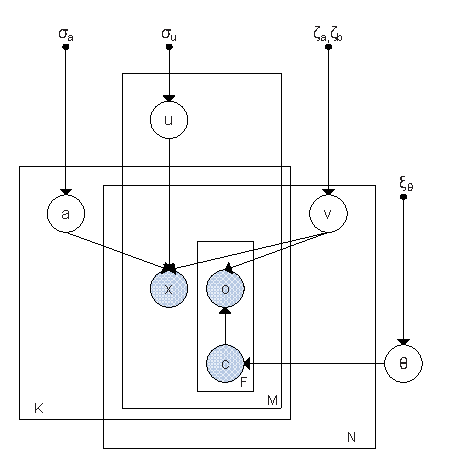
\includegraphics[width=0.3\textwidth]{PGMbasic.eps}
\label{fig:modelbasic}
}
\subfigure[CPV]{
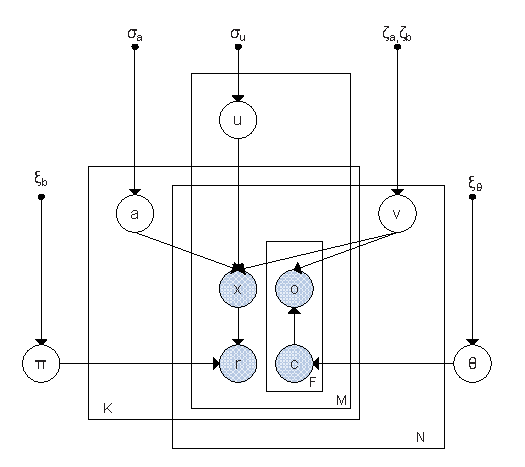
\includegraphics[width=0.3\textwidth]{PGMMNAR.eps}
\label{fig:modelcpv}
}}
\subfigure[CPP ]{
\includegraphics[width=0.3\textwidth]{PGMpref.eps}
\label{fig:modelcpp}
}
\caption{Plate notation for utility models}
\end{figure}




\section{Utility Model with MNAR Observations}\label{sec:mnar}
%the overall framework
The ``absolute'' strategy in model basic is in its essence a model with missing at random observations. When the observations are not missing at random, as shown in Sec.~\ref{sec:method},  the optimal parameters should be inferred by maximizing the joint likelihood of responses and feedback. Depending on the relationship between $x_{u,v,k}$ and $r_{u,v,k}$, we present two models, i.e. conditional probability on the value of feedback (CPV) and conditional probability on the pair-wise preference (CPP).

\subsection{Model CPV}
In model CPV, we assume that the probability of producing a response is dependent on the value of feedback. The conditional probability $p(r|x)$ is denoted as $\Pi$, where $\forall x, \Sigma_r \pi_{r,x}=1, \forall r, \pi_{r,x}>0$. For example, $\pi_{1,1}>\pi_{0,1}$ indicates that users are more willing to brag about a positive purchase. Model CPV has the following generation process.
\begin{itemize}
	\item Generate user preference from a multivariate Gaussian distribution $u\sim \mathcal{N}(u;0,\sigma_u^2)$, contextual preference $a_k\sim \mathcal{N}(a_k;0,\sigma_a^2)$, item specific feature strength $v_c \sim Beta(v_c;\zeta_a,\zeta_b)$ for each user, item-feature, and context respectfully. Generate global vocabulary distribution over the feature phrases $\theta\sim Dirichlet(\theta;\xi)$.
	\item For each review written by $u$ on $v$ under context $k$
	\begin{itemize}
	\item Generate contextual polarity $x\sim Bern(x;g(UC_k(a,u,v)))$
	\item Generate response $r \sim Bern{r;\Pi_x}$
	\item For each product feature
	\begin{itemize}
	\item Choose feature phrases $c\sim Discrete(c;\theta)$
	\item Select an opinion polarity to describe the feature $o \sim Bern(o;v_c)$
	\end{itemize}
	\end{itemize}
\end{itemize}

We apply an EM algorithm for inference. In the M-step, instead of maximizing the expection of joint log-likelihood, we conduct a one-step update along the line search direction. The inference is shown in Alg.~\ref{alg:CPV}.
\begin{algorithm}
\KwIn{A set of positive and negative feedback $\feedback$, a set of feature opinion pairs $\{<c,o>\}$}
\KwOut{$\contextset,\productset,\userset,\Pi$}
Initialize $\contextset,\productset,\userset,\Pi$\;
 \While{not convergent}
{
E-Step\;
\For{$x_{u,v,k}\in \feedback$}
{
	$q(x,u,v,k)=\Pi_{x,1}^{r_{u,v,k}}{(1-\Pi_{x,1})}^{(1-r_{u,v,k})}\frac{1}{1+\exp[(-\alpha \contextk -(1-\alpha)\user)\product]}^{x_{u,v,k}}\frac{\exp[(-\alpha \contextk -(1-\alpha)\user)\product]}{1+\exp[(-\alpha \contextk -(1-\alpha)\user)\product]}^{1-x_{u,v,k}}$\;
	Normalize $q(x,u,v,k)$ over $x\in \{0,1\}$\;
}
M-step\;
\For{$x_{u,v,k}\in \feedback$}
{
		
		$t_{x_{u,v,k},\contextk,\product,\user}= \frac{{\{-\exp{[(-\alpha \contextk -(1-\alpha)\user)\product]}\}}^{x_{u,v,k}}1^{1-x_{u,v,k}}}{1+\exp{[(-\alpha \contextk-(1-\alpha)\user)\product]}}$\;
}
		\For{$\user \in \userset$}
	{
	$\user=\user-\lambda_t [ -(1-\alpha) \Sigma_k \Sigma_{x_{u,v,k}\in \feedback}  t_{x_{u,v,k},\contextk,\product,\user}\product -(1-\alpha) \Sigma_k \Sigma_{x_{u,v,k}\in \feedback^{mis}} \Sigma_{x} q(x,u,v,k)  t_{x_{u,v,k},\contextk,\product,\user}\product -\frac{\user}{\pi\sigma_u^2} ]$\;
	}
	
	\For{$\product \in \productset$}
	{
	$\product=\product-\lambda_t \{\Sigma_k \Sigma_{x_{u,v,k}\in \feedback} [-\alpha \contextk -(1-\alpha)\user] t_{x_{u,v,k},\contextk,\product,\user} + \Sigma_k \Sigma_{x_{u,v,k}\in \feedback^{mis}} [-\alpha \contextk -(1-\alpha)\user] \Sigma_x q(x,u,v,k)t_{x_{u,v,k},\contextk,\product,\user}  + (\zeta_a-1) \product.^{-1}+ (\zeta_b-1) (1-\product).^{-1} \}$\;
	}
	\For{$\contextk \in \contextset$}
	{
	$\contextk=\contextk-\lambda_t [ -\alpha \Sigma_{x_{u,v,k}\in \feedback}  \product t_{x_{u,v,k},\contextk,\product,\user} -\alpha \Sigma_{x_{u,v,k}\in \feedback^{mis}}  \product \Sigma_x q(x,u,v,k) t_{x_{u,v,k},\contextk,\product,\user}  -\frac{\contextk}{\pi \sigma_a^2} ]$\;
	}
	\For{$x \in \{0,1\} $}
	{
	$\Pi_{x,1}=\frac{\Sigma_{x_{u,v,k}\in \feedback}r_{u,v,k}+\Sigma_{x_{u,v,k}\in \feedback^{mis}} q(x,u,v,k) r_{u,v,k}+\zeta_a-1}{|\feedback|+Sigma_{x_{u,v,k}\in \feedback^{mis}} q(x,u,v,k) +\Sigma{j\in {a,b}}(\zeta_j-1)}$\;
	}
}
\caption{Learning Process for model CPV}\label{alg:CPV}
\end{algorithm}

\subsection{Model CPP}
Empirical studies~\cite{Wojnicki2008Word} discovered the phenomenan of extreme reviews. Intuitively, a stronger emotion, either positive or negative, is more likely to trigger a response. In this sense, model CPP explains the generation of extreme reviews by introducing an auxiliary $y_{u,v,k}$, which is the pairwise comparison between contextual and non contextual utility. It assumes that the response is not only related to the contextual utility, but also dependent on the non contextual utility. As shown in Tab.~\ref{tab:CPP}, the reviewers respond to extreme circumstances, i.e. if the user is satisfied with the product under the context $x_{u,v,k}=1$, and the satisfaction is larger than the non contextual satisfaction $y_{u,v,k}=1$, then the user will post a comment;  if the user is disappointed with the product under the context $x_{u,v,k}=0$, and the anger is stronger than the non contextual counterpart $y_{u,v,k}=0$, then a comment is expected; otherwise, the comments will be missing. 
   
\begin{table}
\caption{The NOR distribution of $p(r|x,y)$}\label{tab:CPP}
\centering
\begin{tabular}{|c|c|c|}
\hline\hline
$p(r|x,y)$ & x & y\\\hline
1 & 1 & 1 \\\hline
1 & 0 & 0 \\\hline
0 & 1 & 0 \\\hline
0 & 0 & 1 \\\hline
\hline
\end{tabular}
\end{table}
As shown in Fig.~\ref{fig:models}, we present the following generation process.

\begin{itemize}
	\item Generate user preference from a multivariate Gaussian distribution $u\sim \mathcal{N}(u;0,\sigma_u^2)$, contextual preference $a_k\sim \mathcal{N}(a_k;0,\sigma_a^2)$, item specific feature strength $v_c \sim Beta(v_c;\zeta_a,\zeta_b)$ for each user, item-feature, and context respectfully. Generate global vocabulary distribution over the feature phrases $\theta\sim Dirichlet(\theta;\xi)$.
	\item For each review written by $u$ on $v$ under context $k$
	\begin{itemize}
	\item Generate contextual polarity $x\sim Bern(x;g(UC_k(a,u,v)))$
	\item Generate conventional polarity $y\sim Bern(y;g(UC_k(a,u,v)-UC(u,v)))$
	\item Generate response $r \sim Discrete{\pi}$
	\item For each product feature
	\begin{itemize}
	\item Choose feature phrases $c\sim Discrete(c;\theta)$
	\item Select an opinion polarity to describe the feature $o \sim Bern(o;v_c)$
	\end{itemize}
	\end{itemize}
\end{itemize}

To maximize the likelihood in Equ.~\ref{equ:losspref}, we present the EM algorithm in Alg.~\ref{alg:CPP}. Similar to Alg.~\ref{alg:CPV}, we increase the objective by line search update in the M-step.

\begin{eqnarray}\label{equ:losspref}
 p(\feedback,\response,\mathbf{c},\mathbf{U},\mathbf{V},\mathbf{a}|\mathbf{c},\sigma_u,\sigma_a,\zeta_a,\zeta_b,\xi) & =  \\\nonumber
& \Pi_{x_{u,v,k}\in \feedback}[p(x_{u,v,k}|\mathbf{u,v,a_k})p(y_{u,v,k}=x_{u,v,k}|\mathbf{u,v,a_k})] \\\nonumber
&\Pi_{x_{u,v,k}\in \feedback^{mis}}[\Sigma_x p(x_{u,v,k}=x|\mathbf{u,v,a_k})p(y_{u,v,k}\neq x|\mathbf{u,v,a_k})] \\\nonumber
&p(\mathbf{U}|\sigma_u)p(\mathbf{V}|\zeta_a,\zeta_b)p(\mathbf{a}|sigma_a)\Pi_{o_{c,v}} p(o_{c,v}|c,v)
\end{eqnarray}


\begin{algorithm}
\KwIn{A set of positive and negative feedback $\feedback$, a set of implicit feedback $\feedback^{mis}$, a set of feature opinion pairs $\{<c,o>\}$}
\KwOut{$\contextset,\productset,\userset$}
Initialize $\contextset,\productset,\userset$\;
 \While{not convergent}
{
E-step:
\For{$r_{u,v,k}=0$}
{
\For{$x,y \in \{0,1\}$}
{
 $q(x_{u,v,k},y_{u,v,k})={\frac{1^{x_{u,v,k}}{exp[(-\alpha \user -(1-\alpha)\contextk) \product ]}^{(1-x_{u,v,k})}}{1+exp[(-\alpha \user -(1-\alpha)\contextk) \product ]}}{\frac{1^{y_{u,v,k}}{exp(-\alpha \contextk + \alpha \user)  \product}^{(1-y_{u,v,k})}}{1+exp[(-\alpha \contextk + \alpha \user)  \product]}}p(r_{u,v,k}|x_{u,v,k},y_{u,v,k})$\;
}
Normalize $q(x_{u,v,k},y_{u,v,k}|r_{u,v,k},\product,\user,\contextk)$\;
}
M-step:
\For{$x_{u,v,k}\in \feedback$}
{
		$t_{x_{u,v,k},\contextk,\product,\user}= \frac{{\{-\exp{[(-\alpha \contextk -(1-\alpha)\user)\product]}\}}^{x_{u,v,k}}1^{1-x_{u,v,k}}}{1+\exp{[(-\alpha \contextk-(1-\alpha)\user)\product]}}$\;
		%for y
		$s_{x_{u,v,k},\contextk,\product,\user}= \frac{{\{-\exp{[(-\alpha \contextk + \alpha \user)\product]}\}}^{y_{u,v,k}}1^{1-y_{u,v,k}}}{1+\exp{[(-\alpha \contextk + \alpha \user)\product]}}$\;
}
		\For{$\user \in \userset$}
	{
	$\user=\user-\lambda_t [  \Sigma_k \Sigma_{x_{u,v,k}\in \feedback}  (-(1-\alpha) t_{x_{u,v,k},\contextk,\product,\user}+ \alpha s_{x_{u,v,k},\contextk,\product,\user})\product + \Sigma_k \Sigma_{x_{u,v,k}\in \feedback^{mis}}  \Sigma_{x,y\in \{0,1\}} (-(1-\alpha)q(x,y) q(x_{u,v,k},y_{u,v,k}) t_{x_{u,v,k}=x,\contextk,\product,\user}+\alpha s_{x_{u,v,k}=1-x,\contextk,\product,\user})\product -\frac{\user}{\pi\sigma_u^2} ]$\;
	}
	
	\For{$\product \in \productset$}
	{
	$\product=\product-\lambda_t \{\Sigma_k \Sigma_{x_{u,v,k}\in \feedback} [(-\alpha \contextk -(1-\alpha)\user) t_{x_{u,v,k},\contextk,\product,\user} +(-\alpha \contextk + \alpha \user) s_{x_{u,v,k},\contextk,\product,\user} ]+ \Sigma_k \Sigma_{x_{u,v,k}\in \feedback^{mis}} \Sigma_{x,y\in \{0,1\}}q(x_{u,v,k},y_{u,v,k})[(-\alpha \contextk -(1-\alpha)\user) t_{x_{u,v,k}=x,\contextk,\product,\user} +(-\alpha \contextk + \alpha \user) s_{x_{u,v,k}=1-x,\contextk,\product,\user} ]+ (\zeta_a-1) \product.^{-1}+ (\zeta_b-1) (1-\product).^{-1} \}$\;
	}
	\For{$\contextk \in \contextset$}
	{
	$\contextk=\contextk-\lambda_t [ -\alpha \Sigma_{x_{u,v,k}\in \feedback} [ \product t_{x_{u,v,k},\contextk,\product,\user} -\alpha s_{x_{u,v,k},\contextk,\product,\user} ]+ -\alpha \Sigma_{x_{u,v,k}\in \feedback^{mis}} [\Sigma_{x,y\in\{0,1\}} \product t_{x_{u,v,k},\contextk,\product,\user} -\alpha s_{x_{u,v,k},\contextk,\product,\user} ]q(x_{u,v,k},y_{u,v,k}) -\frac{\contextk}{\pi \sigma_a^2} ]$\;
	}
}
\caption{Learning Process for model CPP}\label{alg:CPP}
\end{algorithm}

\section{Experiment}\label{sec:exp}
In this section, we want to study the following questions. (1) How do we evaluate review guided context aware recommender systems? (2) How does each component of our framework perform, compared with state-of-the-art methods? Towards this end, we design a set of experimental protocals. 

\subsection{Experimental Setup}
We use a  real data set, which is crawled from the largest Chinese review sites\footnote{dianping.com}. We will refer this data set as the dianping data set. We crawl a total number of 2593268 reviews on 15292 restaurants located in Beijing. As shown in figure~\ref{fig:dis}, the review distribution is a truncated power-law distribution. The log probability $logp(k)$ of restaurants with $k$ reviews is linear with $log(k)$. 

\begin{figure}
\subfigure[Distribution of reviews]{
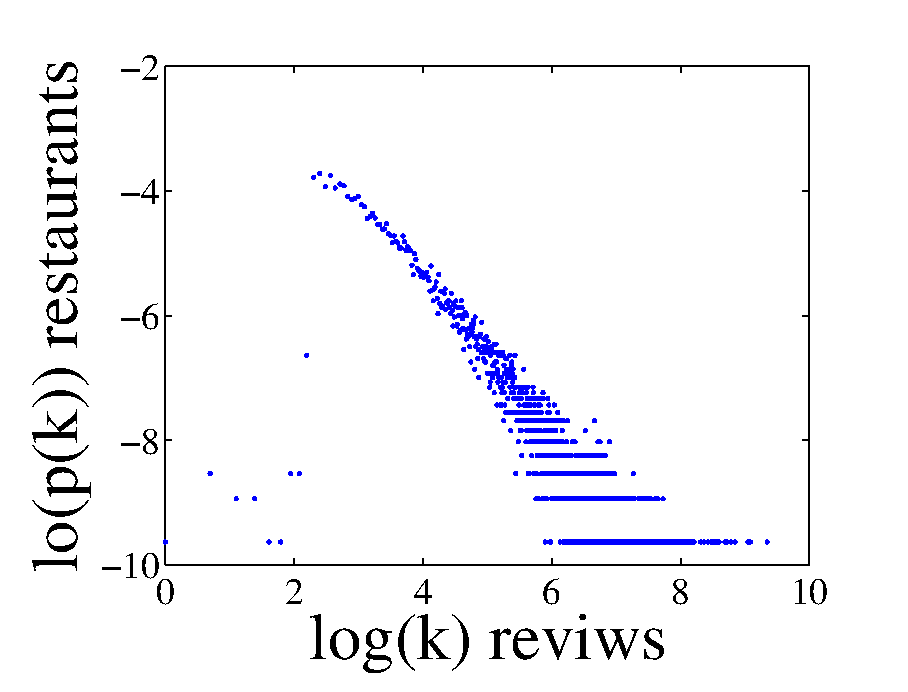
\includegraphics[width=0.5\textwidth]{data.eps}\label{fig:dis}}
\subfigure[Distribution of features]{
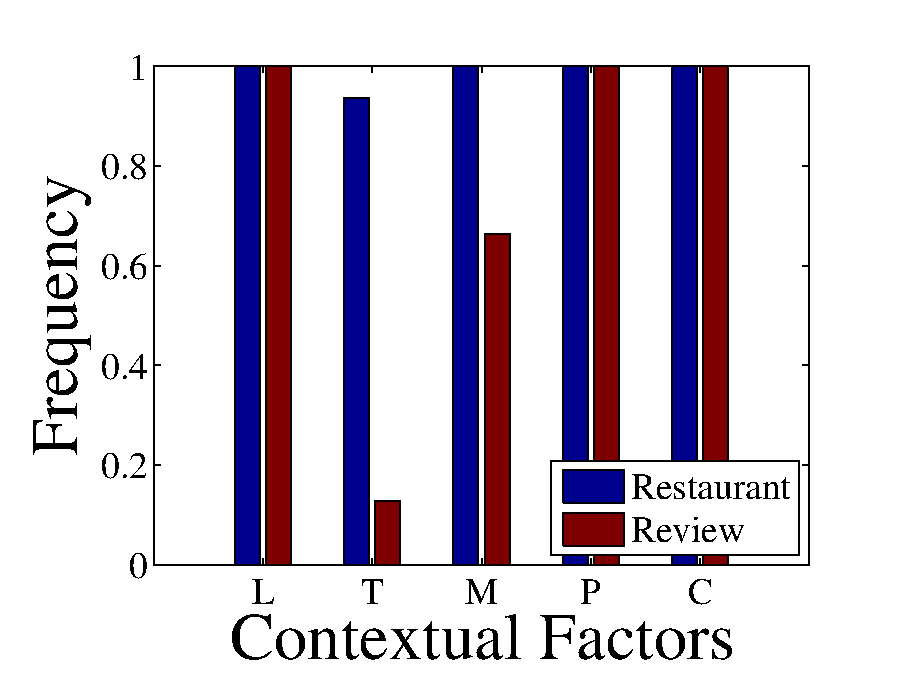
\includegraphics[width=0.5\textwidth]{feature.eps}\label{fig:feat}}
\caption{Statistics of data sets}
\end{figure}

The commodity features are extracted as follows. We first manually build a dictionary containing all the possible aspects of a restaurant, example aspects include ``food'',``parking'',``service'' and so on. Then we run a sentiment classifier~\cite{Liu2005Opinion} to extract the opinion (positive or negative) of the review on each aspect.  Thus the commodity features are pairs consisting of an aspect and an opinion polarity, e.g. ``food+'' is an extracted feature for the following review phrase ``very good food''. In the dianping data set, the price is sometimes demonstrated with the review. In case the price is missing in the review, we use the average price of the restaurant.

The predefined categories for contextual factors used in our experiments include time,location,companion,price and cuisine. We define 5 time factors, including morning, noon, afternoon, night and weekend. Time phrases in a review are matched to one of the 5 time factors. The location factors are collected from dianping, including 43 commercial districts in Beijing. The location factors are identical to all reviews corresponding to the same restaurant. There are 4 types of companion factors(boss, friend, family, couple) and 5 different ranges of number of companions($1,2,3-4,5-10,\geq 10$).The price factors are preprocessed to be 7 categories( $20,20-50,50-80,80-120,120-200,200-500,500-800,\geq 800$). The cuisine factors contain 95 types of cuisines.

All commodity features and contextual factors are binary valued. We count the probability of restaurants and reviews that the contextual factors appear for more than once. As shown in figure~\ref{fig:feat}, cuisine, location and price factors (denoted as ``C'',``L'',and ``P'' in the axis) appear in all restaurants and reviews. A fairy number of people take notes on who they eat with(companion factors denoted as ``M'' in the axis), almost all restaurants have at least one record with companion information. Fewer reviews mention when (time factors denoted as ``T'' in the axis) the experience happens, but the percentage of restaurants with at least one review containing time phrases is much larger.

We define 5 contexts, namely ``Business Banquet'', ``Party'', ``Family Get-together'',`` Dating'' and `` Eat for Leisure''. We pick 27 most popular restaurants and annotate randomly $15\%$ of the reviews (17662 reviews). We observe that the context distribution is unbalanced. Most reviews ($61\%$) are labeled as irrelevant to any context, which suggests the predominance of implicit feedback. $19\%$ reviews are labeled to be positive about  ``Party''. We sample $25\%$ of the size of positive instances from the collection of reviews related to each contexts $\bar{x}$, and construct a relatively balanced negative training set  $E^{-}{x}$, with approximately $125\%$ of the size of $E^{+}{x}$. In annotation and opinion categorization, we only deal with reviews with positive opinions. That is, we first filter out reviews with negative ratings, for a ``cleaner'' training set. 

The step size is set to be $\alpha=1$. The coefficient related to variable std, denoted by $\lambda_p,\lambda_u,\lambda_c$ are decided by cross-validation. For the results below, the values are set to be $\lambda_p=\frac{1}{|E|},\lambda_u=1,\lambda_c=0.01$. The combination weight for contextual and user preference is set to be $\alpha=0.5$.

\subsection{Context Categorization Performance}
We first analyze the capability of the context classification model of selecting the most sensitive factors to each context. Table~\ref{tab:factor} shows the top contextual factors selected with largest $b_{k,f}$ in time, location, companion, number of companions, price and cuisine factors for each context $k$. Consistent with our common sense, people tend to pay more for business banquet and less for a party, arrange datingin weekends, and get together with friends in a party.
\begin{table}\label{tab:factor}
\footnotesize
\centering
\caption{The top contextual factors in each group with the largest $b^x_k$}
\begin{tabular}{|c|c|c|c|c|c|}
  \hline
  % after \\: \hline or \cline{col1-col2} \cline{col3-col4} ...
  Context & Business & Party & Family & Dating & Leisure \\\hline\hline
  Time & noon & afternoon & noon & weekend & weekend \\\hline
  Loc. & E.40th St. & Houhai& Zoo & Sanlitun & Houhai \\\hline
  Comp. & boss & friend & family & family & family \\\hline
  No. Comp. & 5-10 & 3-4 & 3-4 & 2 & 3-4 \\\hline
  Price & 200-500 & 50-80 & 200-500 & 80-120 & 120-200 \\\hline
  Cuisine & roast duck & hotpot &  Russian & ryori & fastfood \\\hline
\end{tabular}
\end{table}


We next analyze how the semi-supervised mechanism improves the categorization. The comparative methods are Naive Bayes, SVM, and Decision Tree. The evaluation metrics are precision and recall rates averaged across all contexts. As shown in Fig.~\ref{fig:classifier}, traditional classifiers suffer from the insufficiency of training instances. The semi-supervision obtains best performance in both metrics. The improvement of precision is in particular significant. Due to the fact of ``silent majority'', a constraint in prior distribution leads to more accurate classification hyperplane. Figure~\ref{fig:KL} shows the KL-divergence of the predicted context distribution and the prior distribution from the annotated reviews of sample size $5\%,10\%,15\%$ respectfully. We can see that the KL-divergence is quite small, and is decreasing as the sample size increases.
\begin{figure}
\centering
\subfigure[Comparative categorization performance]{
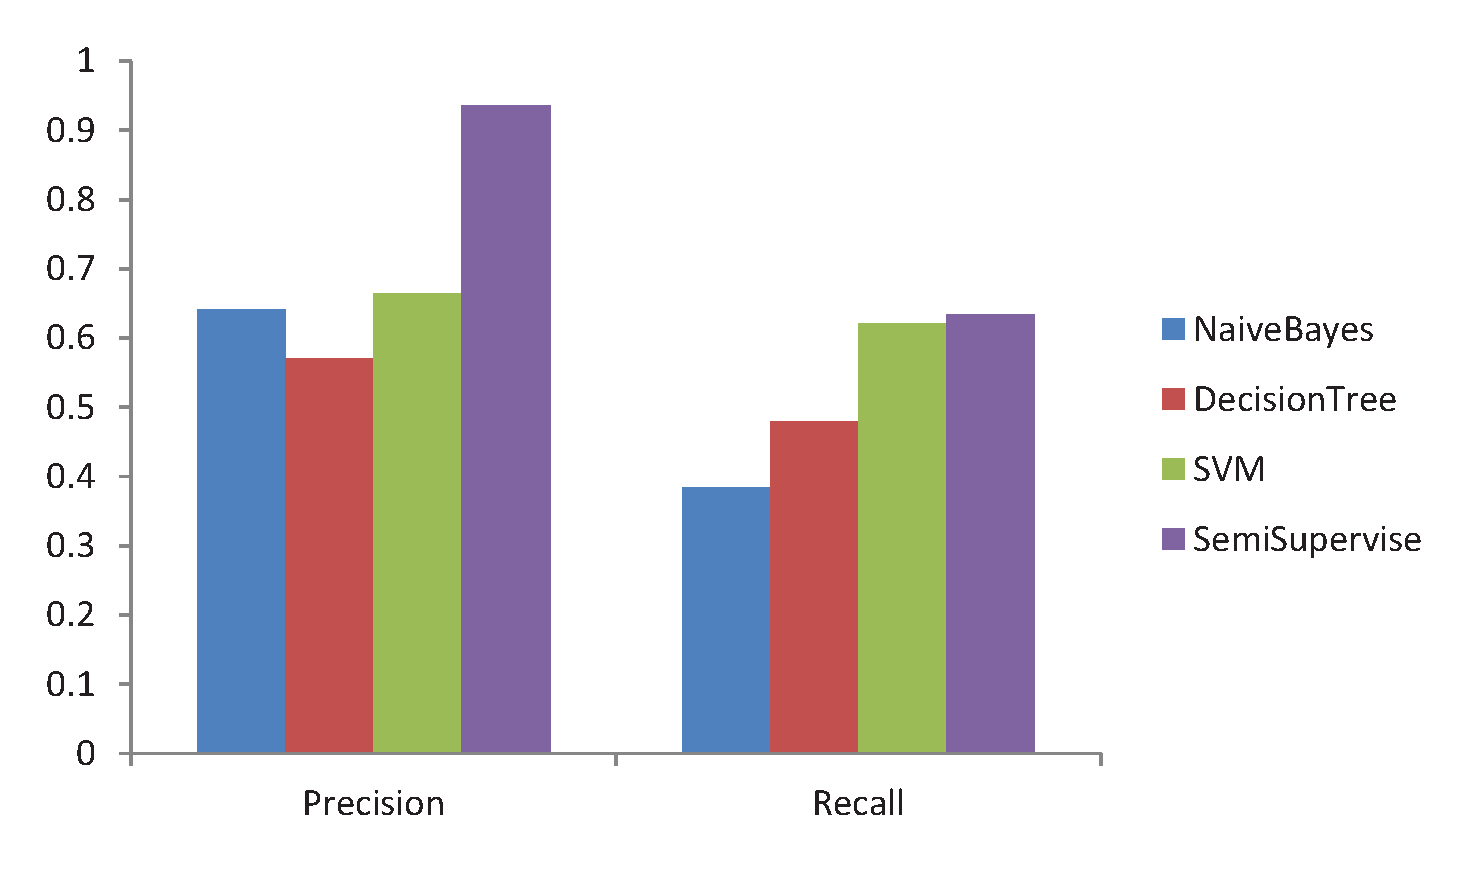
\includegraphics[width=0.45\textwidth]{classifier.eps}\label{fig:classifier}}
\subfigure[$D_{KL}$ with different sample sizes]{
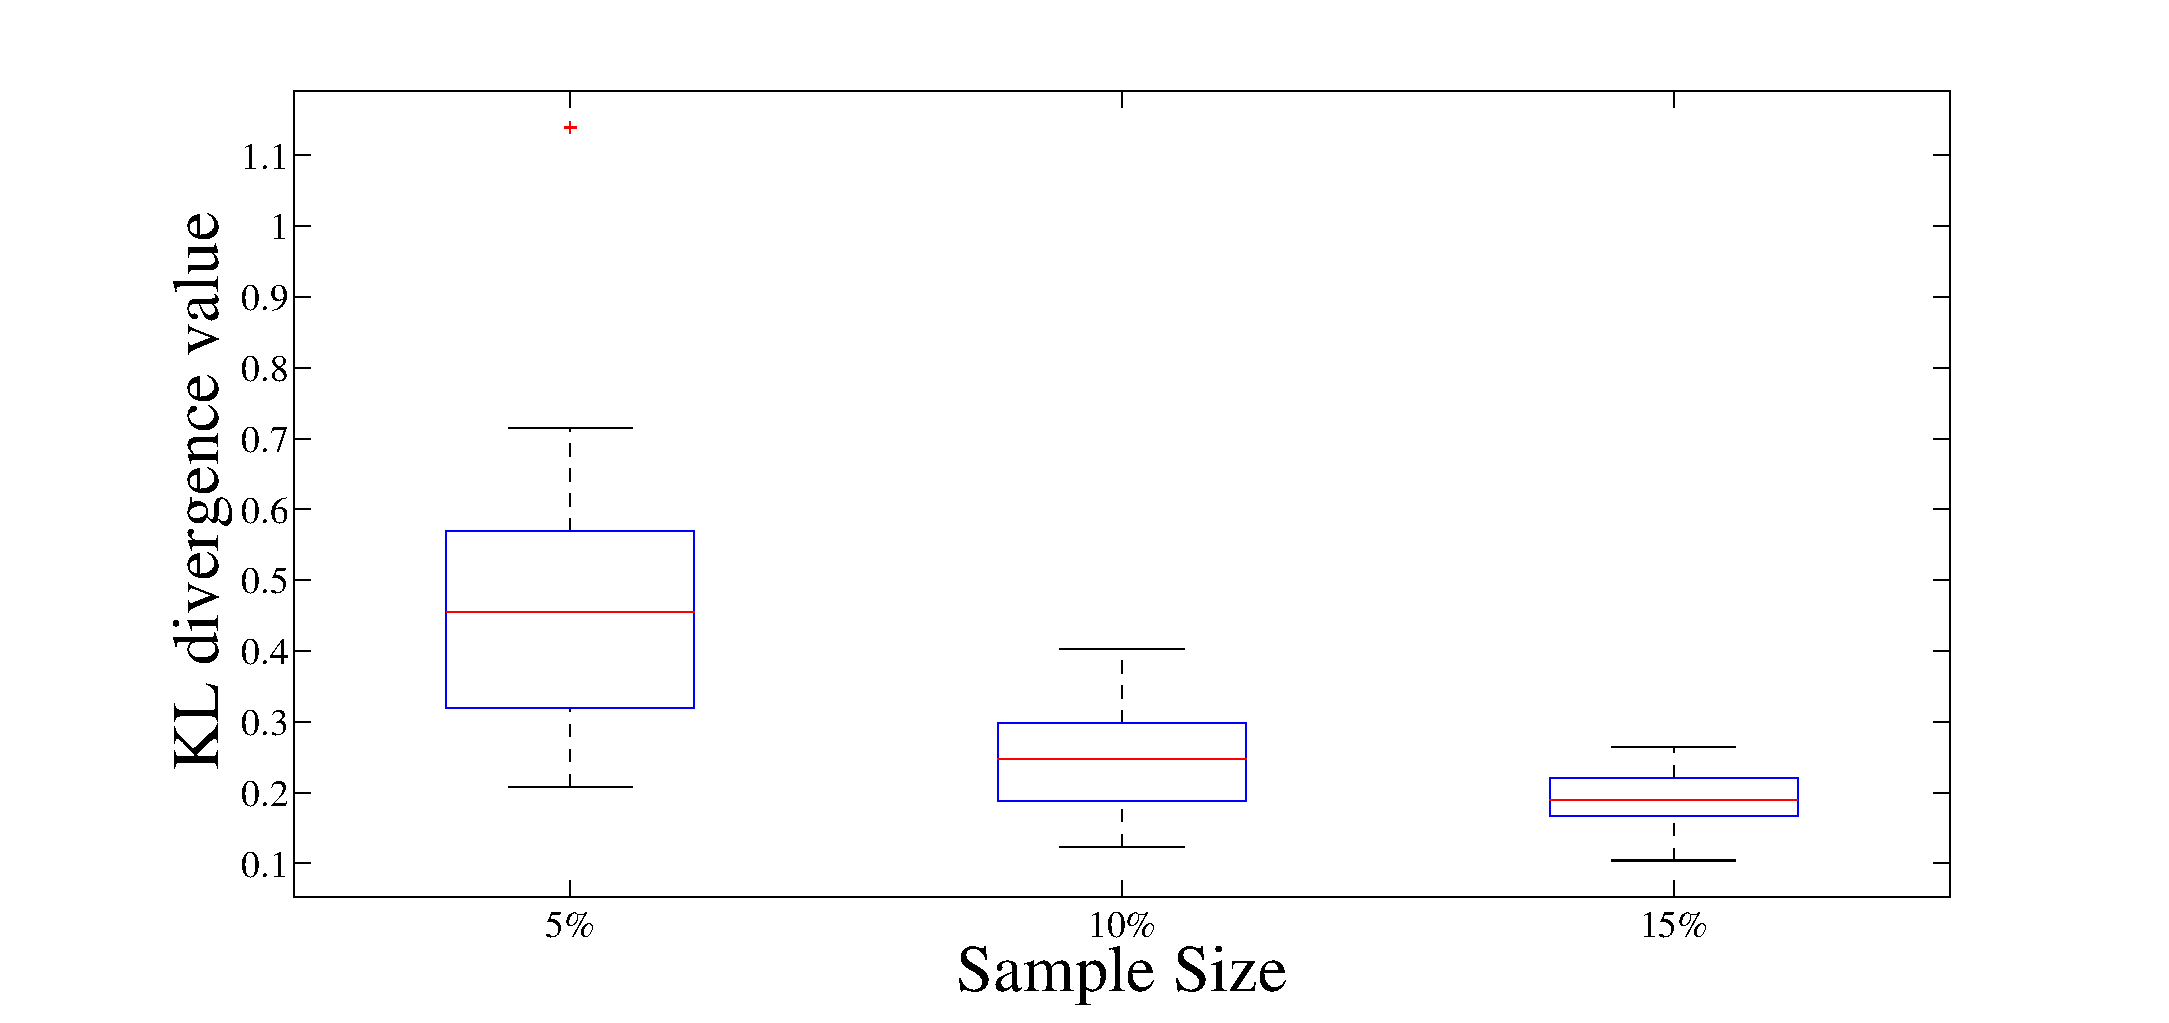
\includegraphics[width=0.45\textwidth]{KL.eps}\label{fig:KL}}
\caption{Performance of contextual categorization}
\end{figure}

\subsection{Cold-start Recommendation}

We next study cold-start recommendation on which most RGCARS focus. We use the intelligent ranking provided by dianping as the gold standard. Precision At Top Ten (P@10) is the evaluation metric. The comparative methods include (1) MostPop, a naive baseline where restaurants are ordered by the number of reviews; (2)TextRating~\cite{Levi2012Finding}, a scoring system based on online review mining; (3)CLDA~\cite{Hariri2013Query}, a LDA alike model for query driven context aware recommendation. We set the query keywords to be the context; (4) our basic model with the ``absolute'' strategy, where $\alpha=1$.


\begin{table}\label{tab:p10}
	\centering
	\caption{Comparative performance of cold-start recommendation}
		\begin{tabular}{|c|c|c|c|c|c|}	
		\hline
Context	&			dating	&business	&family&	party	&leisure\\\hline\hline
MostPop&	0.7&	0.2	&0.1&0.8	&0.1\\\hline
TextRating	&0.6	&0.1	&\textbf{0.2}&	0.4	&0.4\\\hline
CLDA	&\textbf{0.8}	&0.4&	0.1	&0.8&	0.1\\\hline
Basic-absolute	&\textbf{0.8}	&\textbf{0.7}&	\textbf{0.2}&	\textbf{1.0}&	\textbf{1.0}\\\hline
		\end{tabular}
\end{table}

As shown in Tab.~\ref{tab:p10}, our model achieves best results in all contexts, with all pre-procession of textual contents being identical. It shows that the utility surplus model can capture the underlying relationships among user preferences, product features, purchases and reviews. We also notice that utilizing the information in online reviews does not gurantee improvement of the cold-start recommender, especially for context ``business banquet'', ``dating'' and ``party''. This may be caused by the ambiguity of natural language. Erros in extracting the opinions and features from online reviews may cause damage to the recommender. In our model, ratings are important factors for judging the polarity of feedback. Thus our model is more false tolerant to a noisy NLP miner.  

\subsection{Visualization of Context-aware Landmarks}
We pick the top 1000 restaurants computed by basic model in each context. The density of restaurant distribution is drawn at a map of Beijing county. As shown in figure~\ref{fig:lm1} to figure~\ref{fig:lm5}, we have the following observations: (1) the best place for business banquet is right in the city center of Beijing; (2) best places for party are more scattered settled; (3) family can get together at any place, but the famous place of interest Xizhimen is the best choice; (4)dating and leisure eating can also take place at anywhere, but the most popular choice is quite different with that people will make for uniting with family members. The most popular choice Sunlitun is a place full of bars. The visualization accord with our knowledge about the city.
\begin{figure}
\centering
\subfigure[Business]{
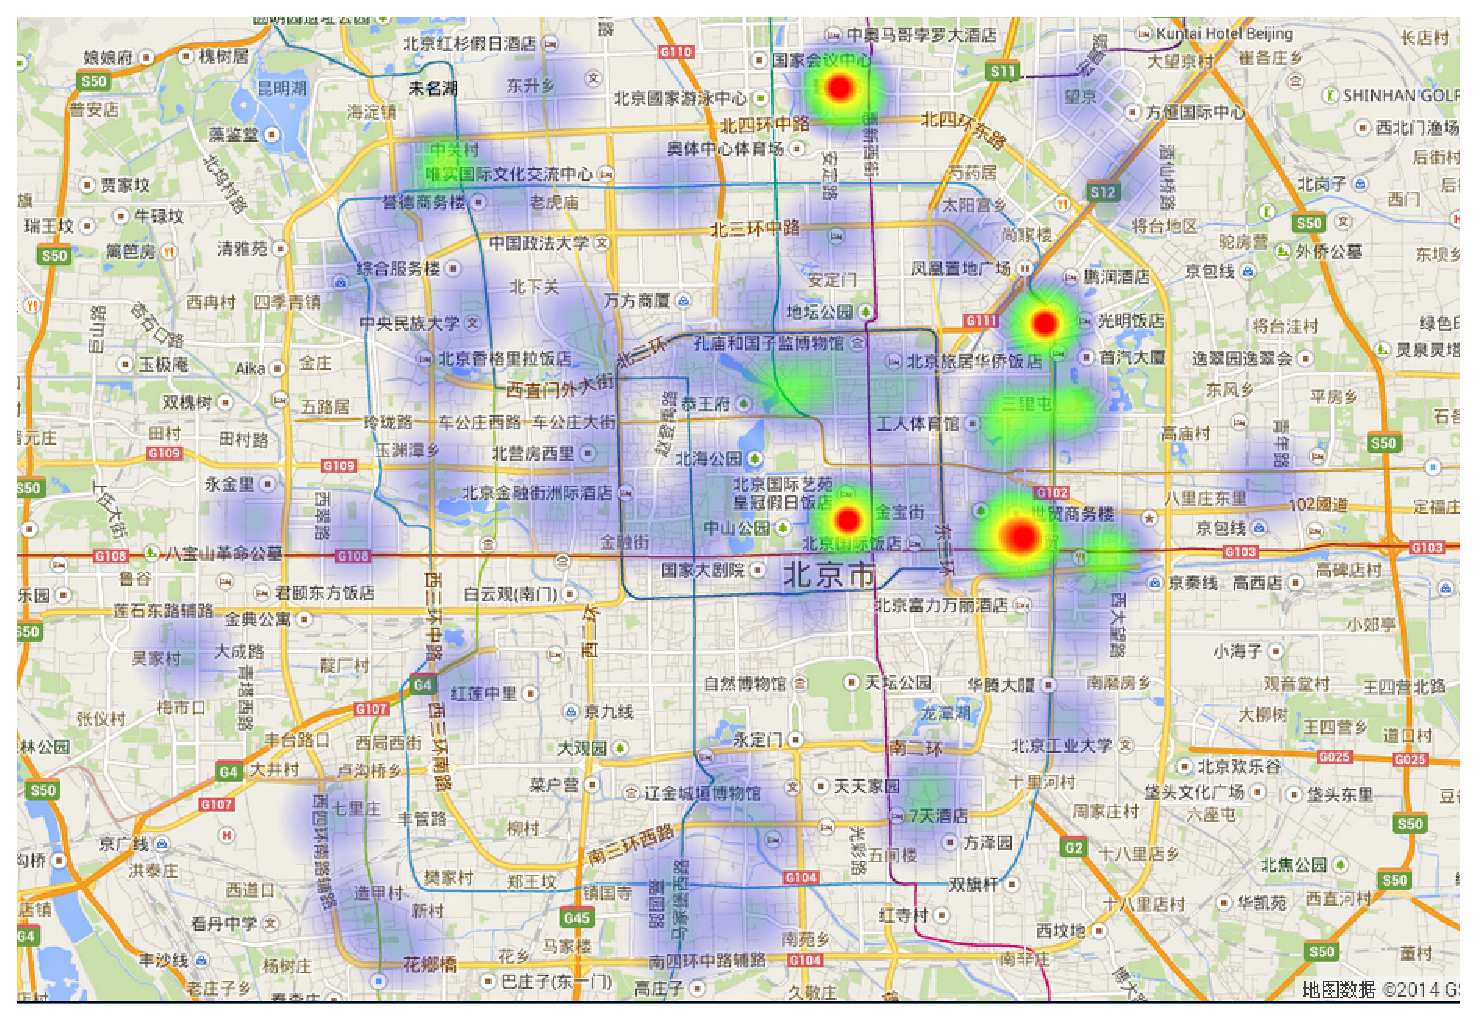
\includegraphics[width=0.45\textwidth]{1.eps}\label{fig:lm1}
}
\subfigure[Party]{
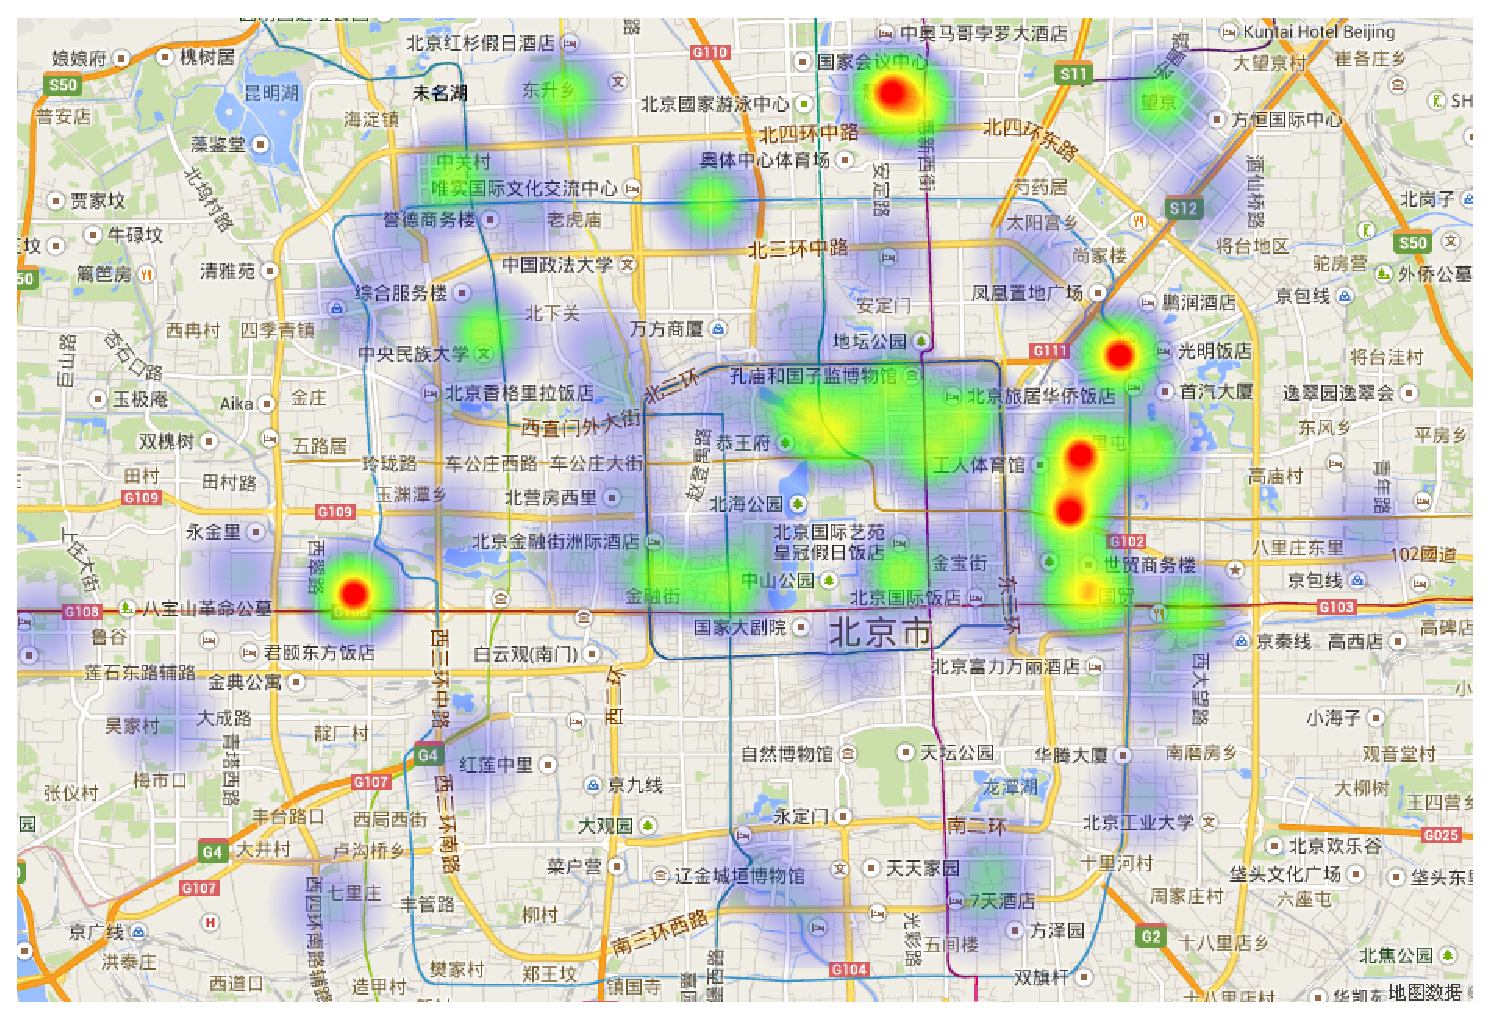
\includegraphics[width=0.45\textwidth]{2.eps}\label{fig:lm2}
}
\subfigure[Family]{
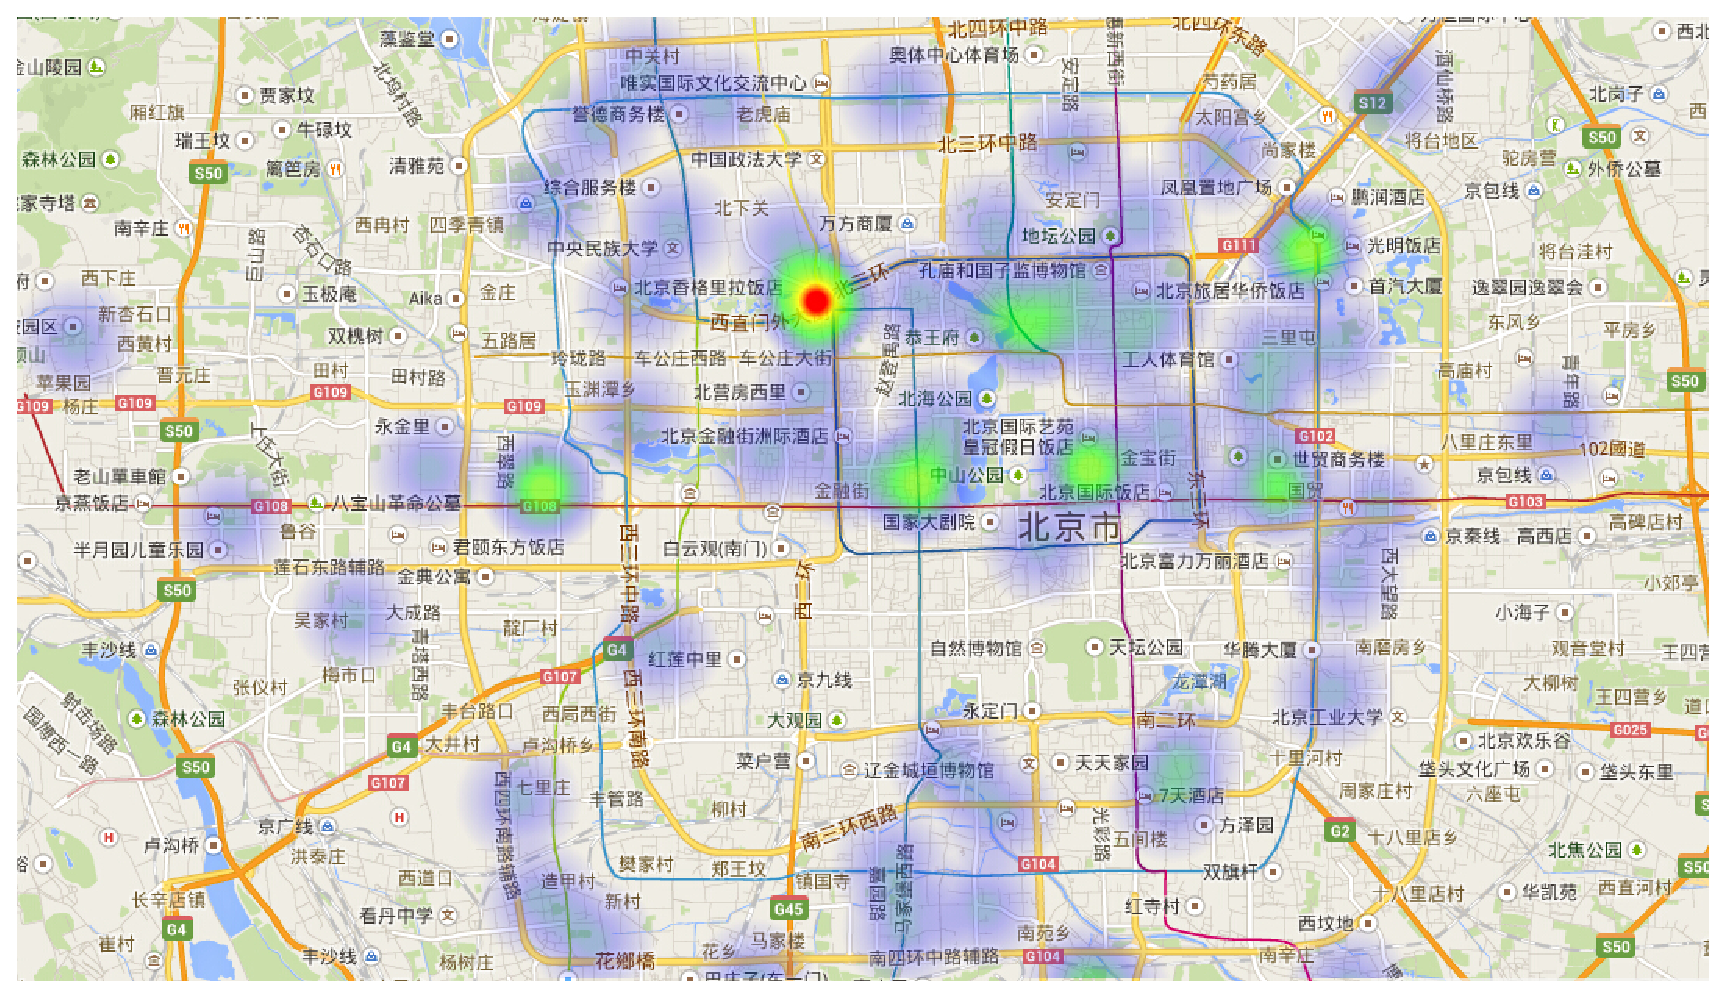
\includegraphics[width=0.45\textwidth]{3.eps}\label{fig:lm3}
}
\subfigure[Dating]{
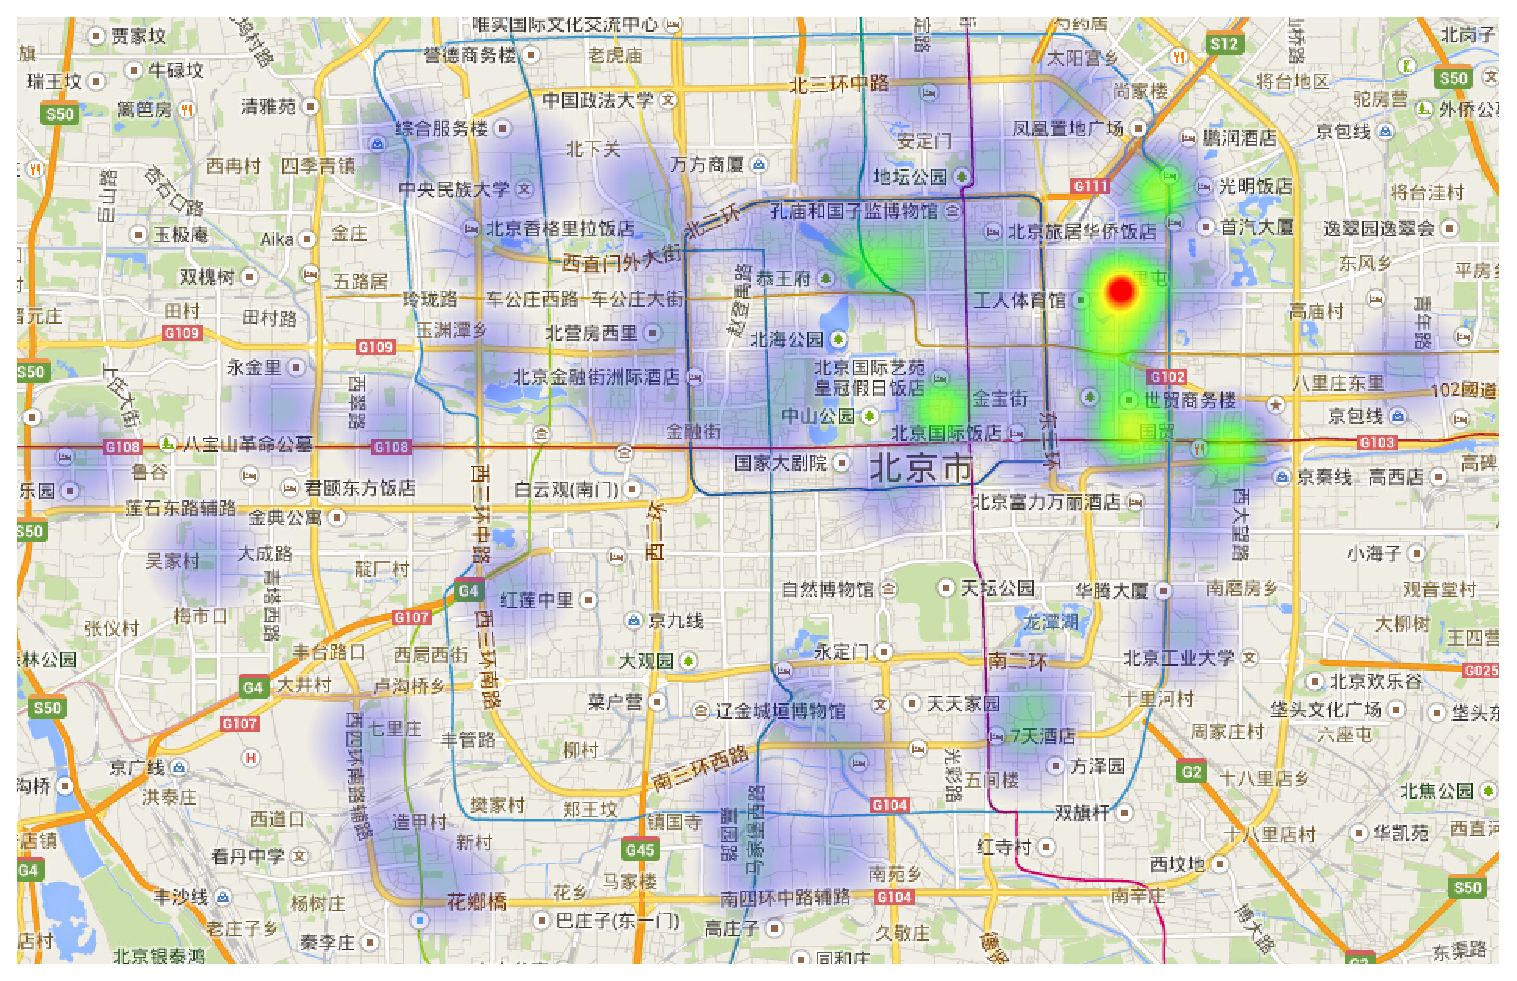
\includegraphics[width=0.45\textwidth]{4.eps}\label{fig:lm4}
}
\subfigure[Leisure]{
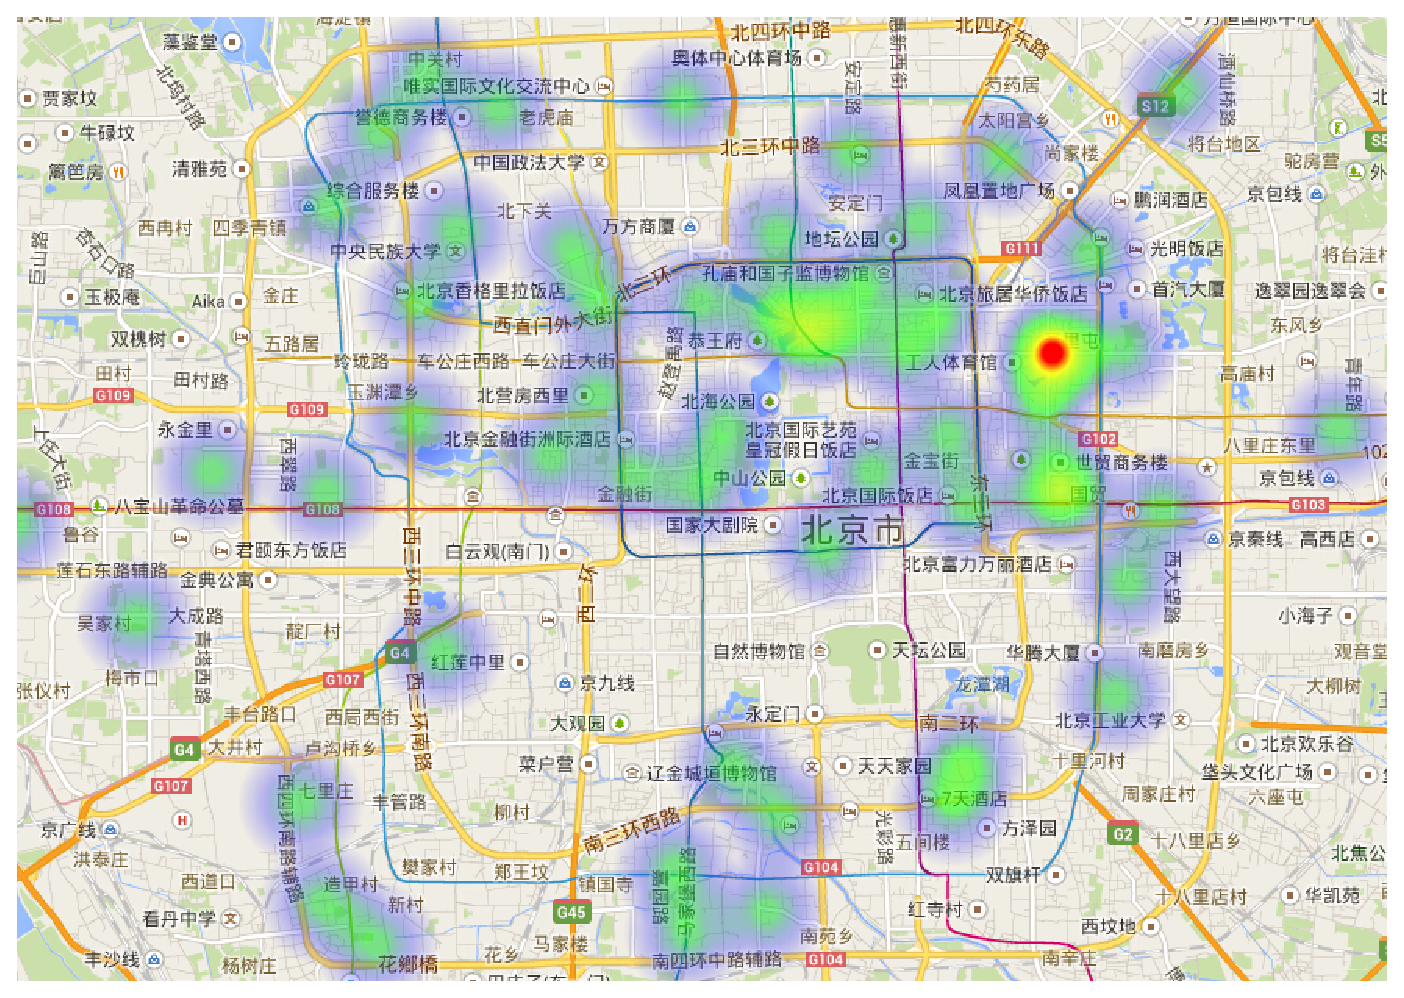
\includegraphics[width=0.45\textwidth]{5.eps}\label{fig:lm5}
}
\caption{Visualization on top 1000 restaurants for each contexts at the map}
\end{figure}


\subsection{Context aware recommendation}
The final task to be evaluated is context aware recommendation. We filter our users with at least 5 reviews for training, and select $10\%$ of the reviews by users with at least 20 reviews for testing. An ideal masurement, for recommendation systems with implicit feedback, is based on predictions of all items for an user, whether they are observed or missing. When such test data is not available, rating based measurements will be imprecise. We use MRR and NDCG as the approximate evaluation metrics. MRR is the mean reciprocal rank of the highest rated restarant of the ground truth in the test set. It is targeted to acquire the best option. NDCG measures quality of the predicted rankings of all ground truth items. We compare our basic models with two strategies (basic-absolute, basic-fuzzy), two variant models (CPV and CPP) with a wide range of state-of-the-art methods, including traditional recommendation models (ItemKNN), models with implicit feedback (CLiMF~\cite{Shi2012CLiMF}, BPR~\cite{Rendle2009BPR}) and models based on online review mining(PLRM~\cite{Li2010Contextual}). The results are plot in Fig.~\ref{fig:mrr} and Fig.~\ref{fig:ndcg}. 

We have the following observations. (1) Our models generally outperform other state-of-the-art methods in terms of MRR and NDCG, for most contexts. Similar to the cold-start recommendation in Tab.~\ref{tab:p10}, our models are significantly better for context ``leisure''. (2) A universal trend exists that models utilizing implicit feedback yield higher results than models which don't, i.e. CliMF and BPR are better than ItemKNN, basic-fuzzy and CPV are better than basic-absolute. This phenomenan highlights the importance of implicit feedback. (3) Compared with CPV, CPP is more sensetive to contexts. As CPP place strict constraints on extreme reviews, it might be more appropriate for less common contexts.   

\begin{figure}[!hbp]
\centering
\subfigure[MRR]{
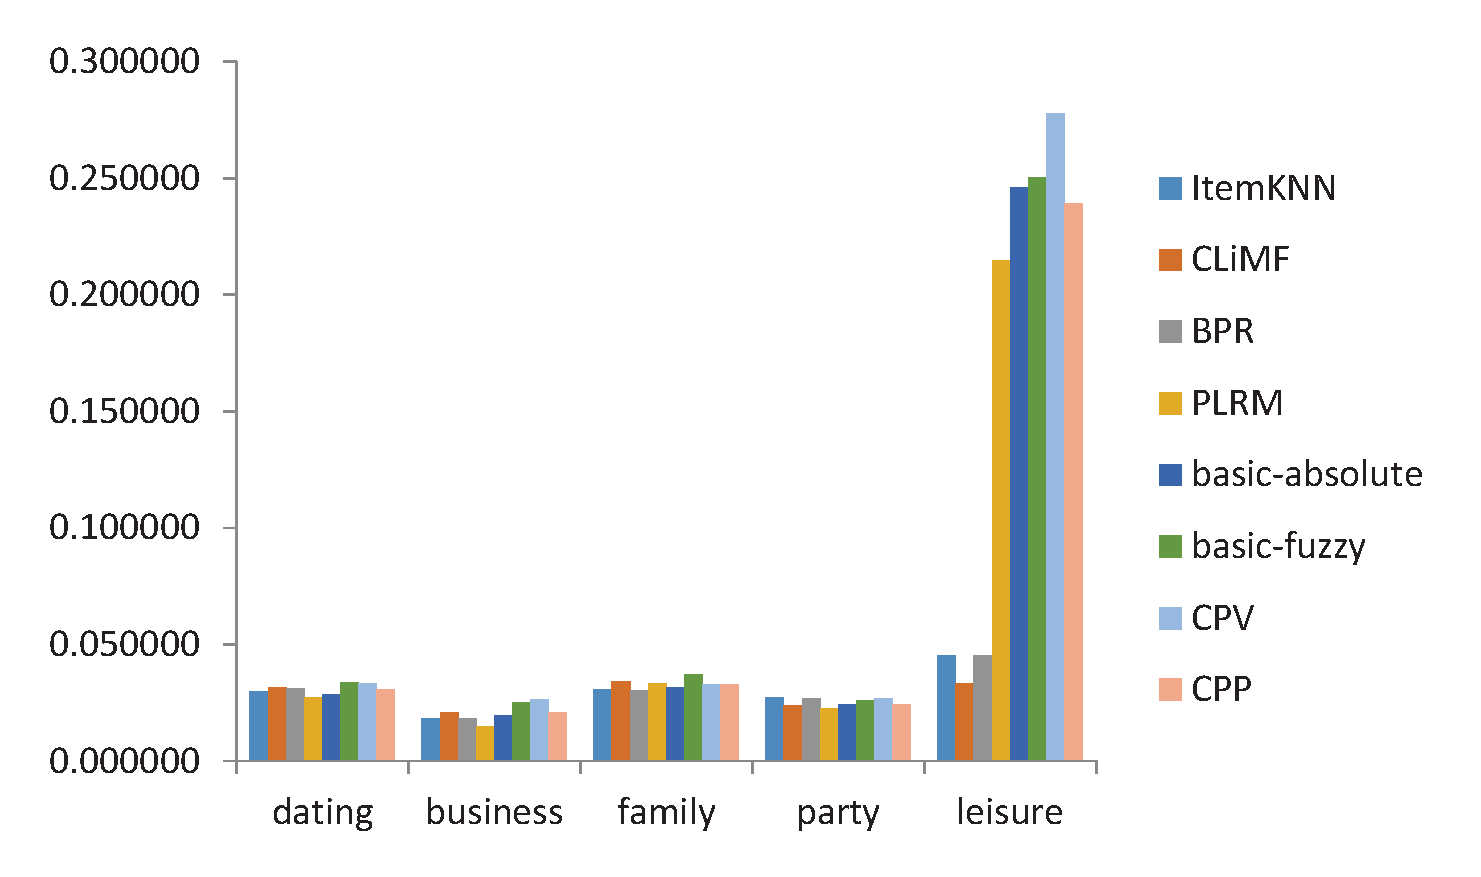
\includegraphics[width=0.45\textwidth]{rankingmrr.eps}\label{fig:mrr}
}
\hspace{0pt}
\vspace{0pt}
\subfigure[NDCG]{
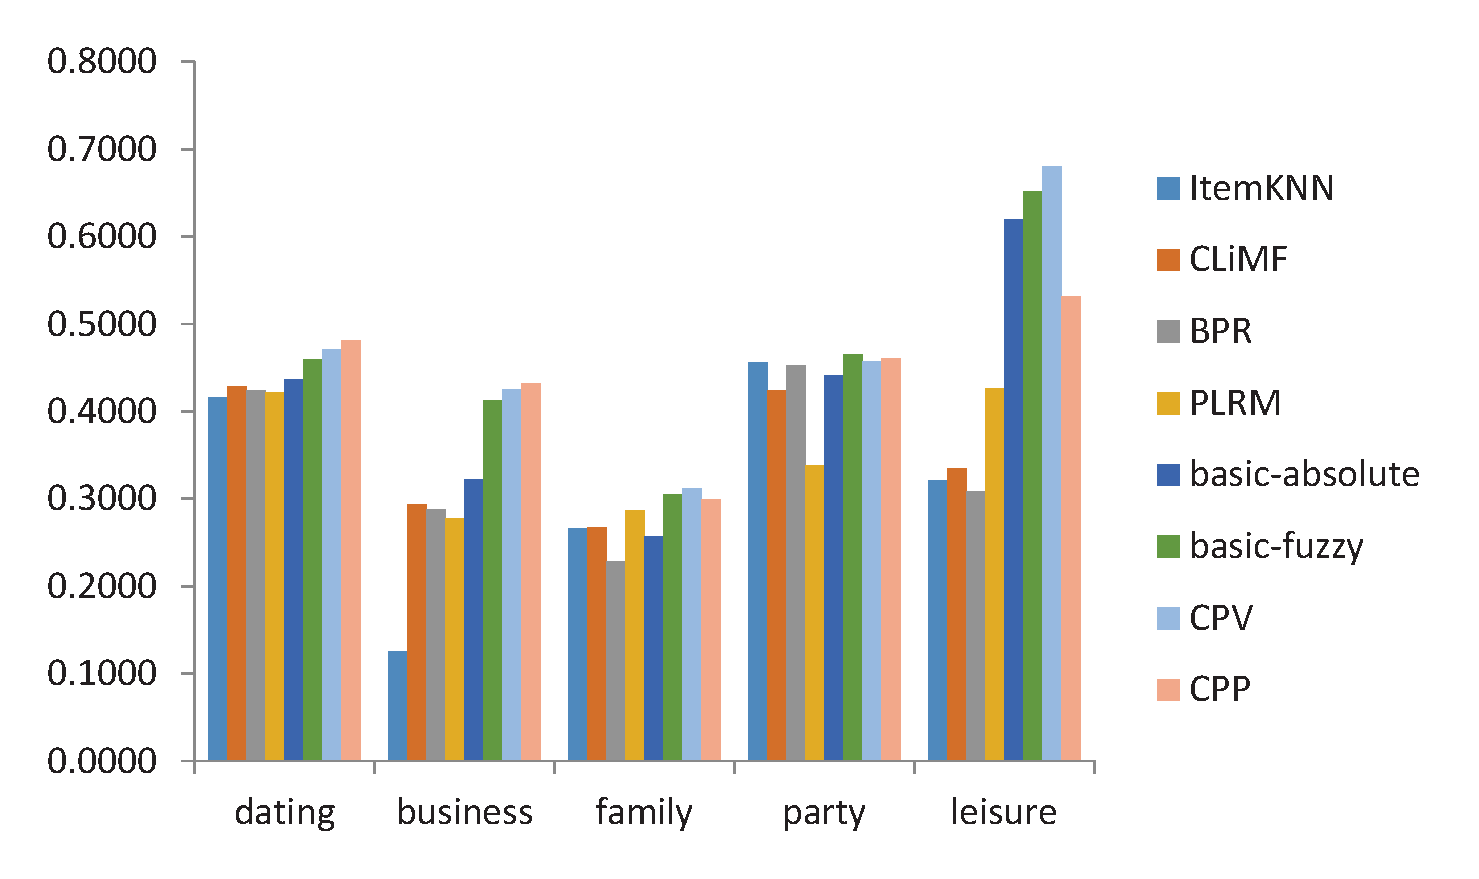
\includegraphics[width=0.45\textwidth]{rankingndcg.eps}\label{fig:ndcg}
}
\caption{Comparative performance of context aware recommender system}
\end{figure}

\section{Conclusion}~\label{sec:con}
In this paper, we mainly focus on exploring the potencial of implicit feedback in a review guided context aware recommender system. We present new models, based on the utility surplus theory,  to tackle the implicit feedback problem by treating them as complete observations or missing not at random observations. We systematically compare the assumptions and performances of thes models.
The most important academic contribution of this paper is that, to the best of our
knowledge, the unique types of implicit feedback (both context free and context aware) have not yet been studied by the community. Therefore our research might shed some insight into mining online reviews for recommender system, and other applications.
Further research issues include adapting and testfying more assumption in the missing not at random model. 
For example, the inter homogenity of online communities, and applying the CPP model to appropriate contexts. 

\section{Acknowledgement}
Chen Lin is partially supported by  China Natural Science Foundation under Grant Nos. NSFC61102136, NSFC61472335, CCF-Tencent Open Research Fund under Grant No. CCF-Tencent20130101, Base Research Project of Shenzhen Bureau of Science,Technology, and Information under Grand No. JCYJ20120618155655087, Baidu Open Research under Grant No.Z153283.

\begin{thebibliography}{10}

\bibitem{Adomavicius2005Incorporating}
Gediminas Adomavicius, Ramesh Sankaranarayanan, Shahana Sen, and Alexander
  Tuzhilin.
\newblock Incorporating contextual information in recommender systems using a
  multidimensional approach.
\newblock {\em ACM Trans. Inf. Syst.}, 23(1):103--145, January 2005.

\bibitem{Adomavicius2011Context}
Gediminas Adomavicius and Alexander Tuzhilin.
\newblock Context-aware recommender systems.
\newblock In {\em Recommender systems handbook}, pages 217--253. Springer,
  2011.

\bibitem{Baltrunas2011Context}
Linas Baltrunas, Bernd Ludwig, Stefan Peer, and Francesco Ricci.
\newblock Context-aware places of interest recommendations for mobile users.
\newblock In {\em Design, User Experience, and Usability. Theory, Methods,
  Tools and Practice}, pages 531--540. Springer, 2011.

\bibitem{Baltrunas2009Context}
Linas Baltrunas and Francesco Ricci.
\newblock Context-based splitting of item ratings in collaborative filtering.
\newblock In {\em Proceedings of the Third ACM Conference on Recommender
  Systems}, RecSys '09, pages 245--248, New York, NY, USA, 2009. ACM.

\bibitem{Bell2007Scalable}
R.M. Bell and Y.~Koren.
\newblock Scalable collaborative filtering with jointly derived neighborhood
  interpolation weights.
\newblock In {\em Data Mining, 2007. ICDM 2007. Seventh IEEE International
  Conference on}, pages 43--52. Ieee, 2007.

\bibitem{Biancalana2013Approach}
Claudio Biancalana, Fabio Gasparetti, Alessandro Micarelli, and Giuseppe
  Sansonetti.
\newblock An approach to social recommendation for context-aware mobile
  services.
\newblock {\em ACM Trans. Intell. Syst. Technol.}, 4(1):10:1--10:31, February
  2013.

\bibitem{Bobadilla2013Recommender}
J.~Bobadilla, F.~Ortega, A.~Hernando, and A.~Guti��rrez.
\newblock Recommender systems survey.
\newblock {\em Knowledge-Based Systems}, 46(0):109 -- 132, 2013.

\bibitem{Cai2007MusicSense}
Rui Cai, Chao Zhang, Chong Wang, Lei Zhang, and Wei-Ying Ma.
\newblock Musicsense: Contextual music recommendation using emotional
  allocation modeling.
\newblock In {\em Proceedings of the 15th International Conference on
  Multimedia}, MULTIMEDIA '07, pages 553--556, New York, NY, USA, 2007. ACM.

\bibitem{Gorgoglione2011Effect}
Michele Gorgoglione, Umberto Panniello, and Alexander Tuzhilin.
\newblock The effect of context-aware recommendations on customer purchasing
  behavior and trust.
\newblock In {\em Proceedings of the Fifth ACM Conference on Recommender
  Systems}, RecSys '11, pages 85--92, New York, NY, USA, 2011. ACM.

\bibitem{Hariri2012Context}
Negar Hariri, Bamshad Mobasher, and Robin Burke.
\newblock Context-aware music recommendation based on latenttopic sequential
  patterns.
\newblock In {\em Proceedings of the Sixth ACM Conference on Recommender
  Systems}, RecSys '12, pages 131--138, New York, NY, USA, 2012. ACM.

\bibitem{Hariri2013Query}
Negar Hariri, Bamshad Mobasher, and Robin Burke.
\newblock Query-driven context aware recommendation.
\newblock In {\em Proceedings of the 7th ACM Conference on Recommender
  Systems}, RecSys '13, pages 9--16, New York, NY, USA, 2013. ACM.

\bibitem{Heckerman1997Models}
David Heckerman and Christopher Meek.
\newblock Models and selection criteria for regression and classification.
\newblock In {\em Proceedings of the Thirteenth Conference on Uncertainty in
  Artificial Intelligence}, UAI'97, pages 223--228, San Francisco, CA, USA,
  1997. Morgan Kaufmann Publishers Inc.

\bibitem{Karatzoglou2010Multiverse}
Alexandros Karatzoglou, Xavier Amatriain, Linas Baltrunas, and Nuria Oliver.
\newblock Multiverse recommendation: N-dimensional tensor factorization for
  context-aware collaborative filtering.
\newblock In {\em Proceedings of the Fourth ACM Conference on Recommender
  Systems}, RecSys '10, pages 79--86, New York, NY, USA, 2010. ACM.

\bibitem{Koren2009Matrix}
Y.~Koren, R.~Bell, and C.~Volinsky.
\newblock Matrix factorization techniques for recommender systems.
\newblock {\em Computer}, 42(8):30--37, 2009.

\bibitem{Levi2012Finding}
Asher Levi, Osnat Mokryn, Christophe Diot, and Nina Taft.
\newblock Finding a needle in a haystack of reviews: Cold start context-based
  hotel recommender system.
\newblock In {\em Proceedings of the Sixth ACM Conference on Recommender
  Systems}, RecSys '12, pages 115--122, New York, NY, USA, 2012. ACM.

\bibitem{Li2011Towards}
Beibei Li, Anindya Ghose, and Panagiotis~G. Ipeirotis.
\newblock Towards a theory model for product search.
\newblock In {\em Proceedings of the 20th international conference on world
  wide web}, pages 327--336, 2011.

\bibitem{Li2010Contextual}
Yize Li, Jiazhong Nie, Yi~Zhang, Bingqing Wang, Baoshi Yan, and Fuliang Weng.
\newblock Contextual recommendation based on text mining.
\newblock In {\em Proceedings of the 23rd International Conference on
  Computational Linguistics: Posters}, COLING '10, pages 692--700, Stroudsburg,
  PA, USA, 2010. Association for Computational Linguistics.

\bibitem{Liu2005Opinion}
Bing Liu, Minqing Hu, and Junsheng Cheng.
\newblock Opinion observer: Analyzing and comparing opinions on the web.
\newblock In {\em Proceedings of the 14th International Conference on World
  Wide Web}, WWW '05, pages 342--351, New York, NY, USA, 2005. ACM.

\bibitem{Liu2013Combining}
Hongyan Liu, Jun He, Tingting Wang, Wenting Song, and Xiaoyang Du.
\newblock Combining user preferences and user opinions for accurate
  recommendation.
\newblock {\em Electronic Commerce Research and Applications}, 12(1):14 -- 23,
  2013.

\bibitem{Moghaddam2013FLDA}
Samaneh Moghaddam and Martin Ester.
\newblock {The FLDA model for aspect-based opinion mining: addressing the cold
  start problem}.
\newblock In {\em Proceedings of the 22nd international conference on World
  Wide Web}, pages 909--918. International World Wide Web Conferences Steering
  Committee, May 2013.

\bibitem{Ounis2006Terrier}
I.~Ounis, G.~Amati, V.~Plachouras, B.~He, C.~Macdonald, and C.~Lioma.
\newblock {Terrier: A High Performance and Scalable Information Retrieval
  Platform}.
\newblock In {\em Proceedings of ACM SIGIR'06 Workshop on Open Source
  Information Retrieval (OSIR 2006)}, 2006.

\bibitem{Palmisano2008Using}
C.~Palmisano, A~Tuzhilin, and M.~Gorgoglione.
\newblock Using context to improve predictive modeling of customers in
  personalization applications.
\newblock {\em Knowledge and Data Engineering, IEEE Transactions on},
  20(11):1535--1549, Nov 2008.

\bibitem{Panniello2009Experimental}
Umberto Panniello, Alexander Tuzhilin, Michele Gorgoglione, Cosimo Palmisano,
  and Anto Pedone.
\newblock Experimental comparison of pre- vs. post-filtering approaches in
  context-aware recommender systems.
\newblock In {\em Proceedings of the Third ACM Conference on Recommender
  Systems}, RecSys '09, pages 265--268, New York, NY, USA, 2009. ACM.

\bibitem{Qu2010Bag}
Lizhen Qu, Georgiana Ifrim, and Gerhard Weikum.
\newblock The bag-of-opinions method for review rating prediction from sparse
  text patterns.
\newblock In {\em Proceedings of the 23rd International Conference on
  Computational Linguistics}, COLING '10, pages 913--921, Stroudsburg, PA, USA,
  2010. Association for Computational Linguistics.

\bibitem{Raghavan2012Review}
Sindhu Raghavan, Suriya Gunasekar, and Joydeep Ghosh.
\newblock Review quality aware collaborative filtering.
\newblock In {\em Proceedings of the Sixth ACM Conference on Recommender
  Systems}, RecSys '12, pages 123--130, New York, NY, USA, 2012. ACM.

\bibitem{Rendle2009BPR}
Steffen Rendle, Christoph Freudenthaler, Zeno Gantner, and Lars Schmidt-Thieme.
\newblock Bpr: Bayesian personalized ranking from implicit feedback.
\newblock In {\em Proceedings of the Twenty-Fifth Conference on Uncertainty in
  Artificial Intelligence}, UAI '09, pages 452--461, Arlington, Virginia,
  United States, 2009. AUAI Press.

\bibitem{salakhutdinov2008probabilistic}
R.~Salakhutdinov and A.~Mnih.
\newblock Probabilistic matrix factorization.
\newblock {\em Advances in neural information processing systems},
  20:1257--1264, 2008.

\bibitem{Shi2012CLiMF}
Yue Shi, Alexandros Karatzoglou, Linas Baltrunas, Martha Larson, Nuria Oliver,
  and Alan Hanjalic.
\newblock Climf: Learning to maximize reciprocal rank with collaborative
  less-is-more filtering.
\newblock In {\em Proceedings of the Sixth ACM Conference on Recommender
  Systems}, RecSys '12, pages 139--146, New York, NY, USA, 2012. ACM.

\bibitem{Shi2010Listwise}
Yue Shi, Martha Larson, and Alan Hanjalic.
\newblock List-wise learning to rank with matrix factorization for
  collaborative filtering.
\newblock In {\em Proceedings of the fourth ACM conference on Recommender
  systems}, RecSys '10, pages 269--272, New York, NY, USA, 2010. ACM.

\bibitem{Si2014Users}
Jianfeng Si, Qing Li, Tieyun Qian, and Xiaotie Deng.
\newblock Users�� interest grouping from online reviews based on topic
  frequency and order.
\newblock In {\em World Wide Web}, 17(6):1321�C1342, 2014.

\bibitem{Wang2015CROWN}
S.~Wang, B.~Zou, C.~Li, K.~Zhao, Q.~Liu, and H.~Chen.
\newblock Crown: A context-aware recommender for web news.
\newblock In {\em 2015 IEEE 31st International Conference on Data Engineering},
  pages 1420--1423, April 2015.
\bibitem{Marlin2009Collaborative}
Marlin, Benjamin M. and Zemel, Richard S.
\newblock Collaborative Prediction and Ranking with Non-random Missing Data
\newblock In {\em Proceedings of the Third ACM Conference on Recommender Systems}, RecSys '09, pages 5--12, New York, NY, USA, 2009, ACM.

\bibitem{Wojnicki2008Word}
\newblock A.C. Wojnicki, D. Godes. 
\newblock Word-of-Mouth as Self-Enhancement
\newblock In {\em HBS Marketing Research Paper No.
06-01}, 2008. 

\end{thebibliography}

\end{document}
